% Options for packages loaded elsewhere
\PassOptionsToPackage{unicode}{hyperref}
\PassOptionsToPackage{hyphens}{url}
\PassOptionsToPackage{dvipsnames,svgnames,x11names}{xcolor}
%

\documentclass[
  fleqn,
  deca,
  blindrev
]{informs4}




\usepackage{amsmath,amssymb}
\usepackage{iftex}
\ifPDFTeX
  \usepackage[T1]{fontenc}
  \usepackage[utf8]{inputenc}
  \usepackage{textcomp} % provide euro and other symbols
\else % if luatex or xetex
  \usepackage{unicode-math}
  \defaultfontfeatures{Scale=MatchLowercase}
  \defaultfontfeatures[\rmfamily]{Ligatures=TeX,Scale=1}
\fi
\usepackage{lmodern}
\ifPDFTeX\else  
    % xetex/luatex font selection
\fi
% Use upquote if available, for straight quotes in verbatim environments
\IfFileExists{upquote.sty}{\usepackage{upquote}}{}
\IfFileExists{microtype.sty}{% use microtype if available
  \usepackage[]{microtype}
  \UseMicrotypeSet[protrusion]{basicmath} % disable protrusion for tt fonts
}{}
\makeatletter
\@ifundefined{KOMAClassName}{% if non-KOMA class
  \IfFileExists{parskip.sty}{%
    \usepackage{parskip}
  }{% else
    \setlength{\parindent}{0pt}
    \setlength{\parskip}{6pt plus 2pt minus 1pt}}
}{% if KOMA class
  \KOMAoptions{parskip=half}}
\makeatother
\usepackage{xcolor}
\setlength{\emergencystretch}{3em} % prevent overfull lines
\setcounter{secnumdepth}{5}
% Make \paragraph and \subparagraph free-standing
\makeatletter
\ifx\paragraph\undefined\else
  \let\oldparagraph\paragraph
  \renewcommand{\paragraph}{
    \@ifstar
      \xxxParagraphStar
      \xxxParagraphNoStar
  }
  \newcommand{\xxxParagraphStar}[1]{\oldparagraph*{#1}\mbox{}}
  \newcommand{\xxxParagraphNoStar}[1]{\oldparagraph{#1}\mbox{}}
\fi
\ifx\subparagraph\undefined\else
  \let\oldsubparagraph\subparagraph
  \renewcommand{\subparagraph}{
    \@ifstar
      \xxxSubParagraphStar
      \xxxSubParagraphNoStar
  }
  \newcommand{\xxxSubParagraphStar}[1]{\oldsubparagraph*{#1}\mbox{}}
  \newcommand{\xxxSubParagraphNoStar}[1]{\oldsubparagraph{#1}\mbox{}}
\fi
\makeatother


\providecommand{\tightlist}{%
  \setlength{\itemsep}{0pt}\setlength{\parskip}{0pt}}\usepackage{longtable,booktabs,array}
\usepackage{calc} % for calculating minipage widths
% Correct order of tables after \paragraph or \subparagraph
\usepackage{etoolbox}
\makeatletter
\patchcmd\longtable{\par}{\if@noskipsec\mbox{}\fi\par}{}{}
\makeatother
% Allow footnotes in longtable head/foot
\IfFileExists{footnotehyper.sty}{\usepackage{footnotehyper}}{\usepackage{footnote}}
\makesavenoteenv{longtable}
\usepackage{graphicx}
\makeatletter
\def\maxwidth{\ifdim\Gin@nat@width>\linewidth\linewidth\else\Gin@nat@width\fi}
\def\maxheight{\ifdim\Gin@nat@height>\textheight\textheight\else\Gin@nat@height\fi}
\makeatother
% Scale images if necessary, so that they will not overflow the page
% margins by default, and it is still possible to overwrite the defaults
% using explicit options in \includegraphics[width, height, ...]{}
\setkeys{Gin}{width=\maxwidth,height=\maxheight,keepaspectratio}
% Set default figure placement to htbp
\makeatletter
\def\fps@figure{htbp}
\makeatother


%%% OPRE uses endnotes. If you do not use them, put a percent sign before
%%% the \theendnotes command. This template does show how to use them.
%\usepackage{endnotes}
%\let\footnote=\endnote
%\let\enotesize=\normalsize
%\def\notesname{Endnotes}%
%\def\makeenmark{$^{\theenmark}$}
%\def\enoteformat{\rightskip0pt\leftskip0pt\parindent=1.75em
%	\leavevmode\llap{\theenmark.\enskip}}

% Private macros here (check that there is no clash with the style)
% figure packages
%\usepackage{graphicx} % already handled in graphics.tex
\usepackage{eqndefns-left}
%\usepackage{multirow} % already handled in tables.tex
\usepackage{hhline}

% caption package
\usepackage[small, margin=1cm]{caption}

% appendix package
\usepackage{appendix}
% color packages
\usepackage{color}
\definecolor{strcolor}{rgb}{0.6, 0.2, 0.6}
\definecolor{commentcolor}{rgb}{0.3125, 0.5, 0.3125}
\definecolor{keycol}{rgb}{0, 0, 1}


% revision
\newcommand{\rev}[1]{{\color{red} #1}}

% math packages
%\usepackage{amssymb}
%\usepackage{amsmath}
\usepackage{bbm}

% Code package
\usepackage{listings}
\lstset{
	emph={ROVar, ROUn, ROVarDR, ROExpr, RONormInf, RONorm1, RONorm2,ROConstraint,ROExpect, ROSq, ROConstraintSet,ROIntVar,ROBinVar, ROInfinity,ROModel,ROVarDRArray, ROVarArray, ROMinimize,ROUnArray, ROAbs, ROPos, ROSum, int},
	emphstyle={\color{strcolor}\bfseries},
	keywordstyle={\color{blue}\bfseries},
	commentstyle={\color{commentcolor}},
	stringstyle={\color{strcolor}\bfseries},
	language=C++,                % choose the language of the code
	basicstyle={\ttfamily\footnotesize}, % the size of the fonts that are used for the code
	numbers=left,                   % where to put the line-numbers
	numberstyle=\footnotesize,      % the size of the fonts that are used for the line-numbers
	stepnumber=1,                   % the step between two line-numbers. If it's 1 each line will be numbered
	numbersep=5pt,                  % how far the line-numbers are from the code
	backgroundcolor=\color{white},  % choose the background color. You must add \usepackage{color}
	showspaces=false,               % show spaces adding particular underscores
	showstringspaces=false,         % underline spaces within strings
	showtabs=false,                 % show tabs within strings adding particular underscores
	frame=single,	                	% adds a frame around the code
	tabsize=2,	                		% sets default tabsize to 2 spaces
	captionpos=b,                   % sets the caption-position to bottom
	breaklines=true,                % sets automatic line breaking
	breakatwhitespace=false,        % sets if automatic breaks should only happen at whitespace
	escapeinside={\%*}{*)},         % if you want to add a comment within your code
	keywords=[1]{for, break, if, else, function}
}
\renewcommand{\lstlistingname}{Code Segment}

% hyperlinks packages
%\usepackage{hyperref}
\usepackage{url}

% numbering
%\numberwithin{equation}{section}
%\numberwithin{table}{section}
%\numberwithin{figure}{section}

% Equation environments
\newcommand {\bea}{\begin{eqnarray}}
	\newcommand {\eea}{\end{eqnarray}}
\newcommand {\E}[1]{\mathrm{E}\left( #1 \right)}
\newcommand {\Ep}[2]{{\mathrm{E}_{\mathbb{P}_{#1}} \left( #2 \right)}}
\newcommand {\supEp}[1]{\displaystyle \sup_{\mathbb{P} \in \mathbb{F}} \Ep{}{#1}}
\newcommand {\supEpf}[2]{\displaystyle \sup_{\mathbb{P} \in \mathbb{F}_{#1}} \Ep{}{#2}}
\newcommand {\pos}[1]{\paren{#1}^+}
\renewcommand {\neg}[1]{\paren{#1}^-}
\newcommand {\pibound}[1]{\ensuremath{\pi^{#1}\paren{r^0, \mb{r}}}}
\newcommand {\etabound}[1]{\ensuremath{\eta^{#1}\paren{r^0, \mb{r}}}}
\newcommand \conv {\mathrm{conv}}
\newcommand {\p}{{\rm P}}
% mb
\newcommand{\mb}[1]{\mbox{\boldmath \ensuremath{#1}}}
\newcommand{\mbt}[1]{\mb{\tilde{#1}}}
\newcommand{\mbb}[1]{\mb{\bar{#1}}}
\newcommand{\mbbs}[1]{\mbb{\scriptstyle{#1}}}
\newcommand{\mbh}[1]{\mb{\hat{#1}}}
\newcommand{\mbth}[1]{\mbt{\hat{#1}}}
\newcommand{\mbc}[1]{\mb{\check{#1}}}
\newcommand{\mbtc}[1]{\mbt{\check{#1}}}
\newcommand{\mbs}[1]{\mb{\scriptstyle{#1}}}
\newcommand{\mbst}[1]{\mbs{\tilde{#1}}}
\newcommand{\mbsh}[1]{\mbs{\hat{#1}}}
% mc
%\newcommand{\mc}[1]{\mbox{\ensuremath{\mathcal{#1}}}}
\newcommand{\mch}[1]{\hat{\mc{#1}}}
\newcommand{\mcs}[1]{\mc{\scriptstyle{#1}}}
\newcommand{\mcss}[1]{\mc{\scriptscriptstyle{#1}}}
\newcommand{\mcsh}[1]{\hat{\mcs{#1}}}
\newcommand{\mbss}[1]{{\mbox{\boldmath \tiny{$#1$}}}}
\newcommand{\eucnorm}[1]{\left\| #1 \right\|_2}
\newcommand{\dpv}{\displaystyle \vspace{3pt}}
\newcommand{\diag}[1]{\textbf{diag}\paren{#1}}
\newcommand{\yldrk}{\mb{y}^k\paren{\mbt{z}}}
\newcommand{\abs}[1]{\left| #1 \right|}
\DeclareMathOperator{\CVaR}{CVaR}
\DeclareMathOperator{\VaR}{VaR}
%\DeclareMathOperator{\argmin}{\arg\min}
% combinations
\renewcommand{\mbc}[1]{\mb{\mc{#1}}}
%misc
\newcommand{\ceil}[1]{\left\lceil #1  \right\rceil}

%\newtheorem{theorem}{Theorem}
%\newtheorem{lemma}[theorem]{Lemma}
\newtheorem{conj}{Conjecture}
\newtheorem{coro}{Corollary}
%\newtheorem{claim}{Claim}
\newtheorem{Defi}{Definition}
\newtheorem{algorithm}{Algorithm}
%\newtheorem{assumption}{Assumption}

\newcommand{\eg}{\textit{e.g.}}
\newcommand{\ie}{\textit{i.e.}}
\renewcommand{\Re}{\mathbb{R}}

%\renewcommand{\bigtimes}{\mathop{\rm \text{\Large{$\times$}}}}

\def\blot{\quad \mbox{$\vcenter{ \vbox{ \hrule height.4pt
				\hbox{\vrule width.4pt height.9ex \kern.9ex \vrule width.4pt}
				\hrule height.4pt}}$}}

% Natbib setup for author-year style
\usepackage{natbib}
\bibpunct[, ]{(}{)}{,}{a}{}{,}%
\def\bibfont{\fontsize{8}{9.5}\selectfont}%
\def\bibsep{0pt}%
\def\bibhang{16pt}%
\def\newblock{\ }%
\def\BIBand{and}%

%% Setup of theorem styles. Outcomment only one.
%% Preferred default is the first option.
\TheoremsNumberedThrough     % Preferred (Theorem 1, Lemma 1, Theorem 2)
%\TheoremsNumberedByChapter  % (Theorem 1.1, Lema 1.1, Theorem 1.2)
\ECRepeatTheorems

%% Setup of the equation numbering system. Outcomment only one.
%% Preferred default is the first option.
\EquationsNumberedThrough    % Default: (1), (2), ...
%\EquationsNumberedBySection % (1.1), (1.2), ...

% In the reviewing and copyediting stage enter the manuscript number.
%\MANUSCRIPTNO{} % When the article is logged in and DOI assigned to it,
%   this manuscript number is no longer necessary

%\newdimen\setvrulersecondcolumnheightdimen%
%\newbox\setvrulersecondcolumnheightdimenbox%
%%%%%%%%%%%%%%%%%
\gdef\AQ#1{}
\gdef\CQ#1{}
\usepackage{booktabs}
\usepackage{longtable}
\usepackage{array}
\usepackage{multirow}
\usepackage{wrapfig}
\usepackage{float}
\usepackage{colortbl}
\usepackage{pdflscape}
\usepackage{tabu}
\usepackage{threeparttable}
\usepackage{threeparttablex}
\usepackage[normalem]{ulem}
\usepackage{makecell}
\usepackage{xcolor}
%% Uncomment a line to change font and spacing
%\SingleSpacedXI % 11pt and 1x line spacing
%\SingleSpacedXII % 12pt and 1x line spacing
%\OneAndAHalfSpacedXI % 11pt and 1.5x line spacing
\OneAndAHalfSpacedXII % 12pt and 1.5x line spacing
%\DoubleSpacedXI % 11pt and 2x line spacing
%\DoubleSpacedXII % 12pt and 2x line spacing
\usepackage{orcidlink}
\definecolor{mypink}{RGB}{219, 48, 122}
\makeatletter
\@ifpackageloaded{caption}{}{\usepackage{caption}}
\AtBeginDocument{%
\ifdefined\contentsname
  \renewcommand*\contentsname{Table of contents}
\else
  \newcommand\contentsname{Table of contents}
\fi
\ifdefined\listfigurename
  \renewcommand*\listfigurename{List of Figures}
\else
  \newcommand\listfigurename{List of Figures}
\fi
\ifdefined\listtablename
  \renewcommand*\listtablename{List of Tables}
\else
  \newcommand\listtablename{List of Tables}
\fi
\ifdefined\figurename
  \renewcommand*\figurename{Figure}
\else
  \newcommand\figurename{Figure}
\fi
\ifdefined\tablename
  \renewcommand*\tablename{Table}
\else
  \newcommand\tablename{Table}
\fi
}
\@ifpackageloaded{float}{}{\usepackage{float}}
\floatstyle{ruled}
\@ifundefined{c@chapter}{\newfloat{codelisting}{h}{lop}}{\newfloat{codelisting}{h}{lop}[chapter]}
\floatname{codelisting}{Listing}
\newcommand*\listoflistings{\listof{codelisting}{List of Listings}}
\makeatother
\makeatletter
\makeatother
\makeatletter
\@ifpackageloaded{caption}{}{\usepackage{caption}}
\@ifpackageloaded{subcaption}{}{\usepackage{subcaption}}
\makeatother
\ifLuaTeX
  \usepackage{selnolig}  % disable illegal ligatures
\fi
\usepackage[]{natbib}
\bibliographystyle{informs2014}
\usepackage{bookmark}

\IfFileExists{xurl.sty}{\usepackage{xurl}}{} % add URL line breaks if available
\urlstyle{same} % disable monospaced font for URLs
\hypersetup{
  pdftitle={Quantile-parameterized distributions for expert knowledge elicitation},
  pdfauthor={Dmytro Perepolkin; Erik Lindström; Ullrika Sahlin},
  pdfkeywords={quantile functions, quantile-parameterized
distributions, expert knowledge elicitation, statistical distributions},
  colorlinks=true,
  linkcolor={blue},
  filecolor={Maroon},
  citecolor={Blue},
  urlcolor={Blue},
  pdfcreator={LaTeX via pandoc}}


%	\AIA
% \setcounter{page}{1} %
% \VOL{0}%
% \NO{0}%
% \MONTH{Xxxxx}%
% \YEAR{2024}%
% \FIRSTPAGE{1}%
% \LASTPAGE{16}%
% \FIRSTPAGEAIA{1}%
% \LASTPAGEAIA{16}%
\def\COPYRIGHTHOLDER{INFORMS}%
\def\COPYRIGHTYEAR{2024}%


%\def\RECEIVED{November 1, 2016}
%\def\REVISED{June 22, 2017; October 6, 2017}
%\def\ACCEPTED{November 15, 2017}
% \PUBONLINEAIA{}
	\RUNAUTHOR{Perepolkin et al.} %

	\RUNTITLE{QPDs for EKE}
\TITLE{Quantile-parameterized distributions for expert knowledge
elicitation}

\ARTICLEAUTHORS{
\AUTHOR{Dmytro Perepolkin}\AFF{Lund University, Centre for Environmental
and Climate Science}
\AUTHOR{Erik Lindström}\AFF{Lund University, Centre for Mathematical
Sciences}
\AUTHOR{Ullrika Sahlin}\AFF{Lund University, Centre for Environmental
and Climate Science}
}
%\date{}%
\FUNDING{U Sahlin was funded by the Crafoord Foundation (ref 20200626).}


\AREAOFREVIEW{Decision Analysis}

\KEYWORDS{quantile functions; quantile-parameterized
distributions; expert knowledge elicitation; statistical distributions}

\begin{document}
\ABSTRACT{This paper provides a comprehensive overview of
quantile-parameterized distributions (QPDs) as a tool for capturing
expert predictions and parametric judgments. We survey a range of
methods for constructing distributions that are parameterized by a set
of quantile-probability pairs and describe an approach to generalizing
them to enhance their tail flexibility. Furthermore, we delve into the
extension of QPDs to the multivariate setting, surveying the approaches
to construct bivariate distributions, which can be adopted to obtain
distributions with quantile-parameterized margins. Through this review
and synthesis of the previously proposed methods, we aim to enhance the
understanding and utilization of QPDs in various domains.}
\maketitle

\section{Introduction}\label{introduction}

Judgment plays a crucial role in transforming raw data into meaningful
insights. To be useful, judgment must be translated into mathematical
models and assumptions. These models are designed to capture the
expert's understanding of the world, including the causal links between
relevant entities. The models serve as a representation of this
understanding, while also addressing knowledge limitations, treated as
uncertainties. Elicitation involves translating qualitative
understanding into quantitative models offering valuable insights.

\subsection*{Past research}\label{past-research}
\addcontentsline{toc}{subsection}{Past research}

Most of the expert elicitation protocols described in the literature
\citep{hanea2021ExpertJudgementRisk, gosling2018SHELFSheffieldElicitation, ohagan2006UncertainJudgementsEliciting, hemming2018PracticalGuideStructured, morgan2014UseAbuseExpert, welsh2018MoreorlessElicitationMOLE, spetzler1975ProbabilityEncodingDecision}
encode expert judgments about the parameter or quantity of interest as
an ordered set of quantiles with corresponding probabilities. This
typically includes measures such as the median and the upper and lower
quartiles. Assessors are then encouraged to select a probability
distribution that reasonably fits the elicited quantile-probability
pairs and validate the choice with the expert
\citep{gosling2018SHELFSheffieldElicitation}. A distribution is selected
from a predefined set of ``simple and convenient'' distributions
\citep{ohagan2006UncertainJudgementsEliciting} with boundedness that
accounts for the nature of the elicited quantity.

Several specialized distributions have been developed to facilitate
smooth interpolation of probabilistic assessments. These distributions,
parameterized by quantile-probability pairs, ensure that the elicited
quantile-probability pairs (QPPs) are exactly preserved
\citep{keelin2011QuantileParameterizedDistributions, powley2013QuantileFunctionMethods, keelin2016MetalogDistributions, hadlock2017QuantileparameterizedMethodsQuantifying, wilson2023ReconciliationExpertPriors}.
Quantile-parameterized distributions are particularly valuable thanks to
the interpretability of their parameters. By leveraging the elicited
quantiles, these distributions enable precise capturing of expert
knowlegde while maintaining a high level of flexibility in modeling.

We believe that the primary utility of QPDs lies in their ability to
simplify the specification of probability distributions for model
parameters, known as \emph{prior elicitation}
\citep{mikkola2021PriorKnowledgeElicitation}. However, these same
distributions can also be employed to describe an expert's predictions
for the next observation, referred to as \emph{predictive elicitation}
\citep{winkler1980PriorInformationPredictive, kadane1980PredictiveStructuralMethods, akbarov2009ProbabilityElicitationPredictive, hartmann2020FlexiblePriorElicitation},
or to capture both uncertainty and variability through a two-dimensional
probability distribution in \emph{hybrid elicitation}
\citep{perepolkin2021HybridElicitationIndirect}.

This review paper aims to introduce quantile-parameterized distributions
(QPDs) to a wide readership. The literature review and the findings are
presented through the perspective of quantile functions, building upon
the theoretical foundations established by Parzen
\citep{parzen1979NonparametricStatisticalData} and Gilchrist
\citep{gilchrist2000StatisticalModellingQuantile}. The derivatives and
inverses for each of the quantile functions discussed in the paper are
provided in Appendix A, serving as a valuable reference for future
research. Through our comprehensive review and identification of
research gaps, we aim to contribute to the development of flexible and
extensible distributions that can effectively capture expert knowledge.
We hope that our overview of quantile-parameterized distributions will
be useful for researchers and practitioners, enabling them to make an
informed choice of a distribution suitable for the task.

\subsection*{Paper structure}\label{paper-structure}
\addcontentsline{toc}{subsection}{Paper structure}

In Section 2, we revisit the approaches to quantile parameterization of
probability distributions and explore how QPDs can effectively describe
expert beliefs regarding model parameters or predictions. In Section 3,
we conduct a comprehensive review and comparison of various continuous
univariate QPDs found in the literature. Specifically, we focus on the
Myerson distribution and its generalization accommodating different tail
thicknesses. We compare the robust moments of QPDs to assess their
flexibility and behavior. This comparative analysis can guide the
selection of an appropriate distribution to characterize the quantity of
interest. In Section 4, we explore several methods for extending
univariate distributions to a multivariate setting. These methods
include the utilization of standard multivariate distributions
\citep{drovandi2011LikelihoodfreeBayesianEstimation}, copulas
\citep{hoff2007ExtendingRankLikelihood}, and bivariate quantiles
\citep{nair2023PropertiesBivariateDistributions, vineshkumar2019BivariateQuantileFunctions}.
We show how these techniques can be applied to develop a bivariate
version of the Generalized Myerson distribution and demonstrate its
application in parametric and predictive elicitation. Finally, in
Section 5, we discuss future research directions and potential
applications of QPDs in Bayesian analysis.

\section{Quantile parameterization of probability
distributions}\label{quantile-parameterization-of-probability-distributions}

A fundamental principle in Bayesian data analysis is that learning from
data involves more than formulating hypotheses and models. It
necessitates articulating prior beliefs, expressing existing knowledge
mathematically, and translating it into probability distributions for
model parameters.

To accurately translate knowledge into the language of statistical
models the encoding distribution needs to be flexible, the process
should be transparent, and the results must be interpretable. For
continuous distributions, elicitation often consists of capturing a
series of quantile-probability pairs (QPPs)
\citep{kadane1998ExperiencesElicitation, morgan2014UseAbuseExpert}, and
then fitting a distribution to these pairs
\citep{ohagan2019ExpertKnowledgeElicitation}. However, in practice, the
choice of a parametric distribution to fit the elicited QPPs is often
influenced by concerns about conjugacy with the selected statistical
model that represents the data-generative process (the likelihood
function) and/or the availability of required distribution functions and
fitting algorithms in the software employed. Frequently, the selected
distribution possesses fewer parameters than the number of elicited
QPPs, which can result in a less-than-perfect fit
\citep{ohagan2019ExpertKnowledgeElicitation}. For instance, it is common
to elicit three quantiles (the median along with an upper and lower
quartile) and subsequently attempt to fit a normal or lognormal
distribution (which features two parameters) to these points.

An alternative approach to characterizing the distribution of
predictions or parameters is through quantile-parameterized
distributions (QPDs). These distributions are parameterized by the QPPs,
allowing the elicited values to directly define the distribution,
thereby ensuring a good fit and interpretability of parameters. The QPDs
examined in this paper can accommodate a wide range of shapes and
boundedness, making them valuable for accurately representing experts'
prior beliefs.

Parameterizing distributions using a vector of quantiles is not a novel
concept in the scientific community. The earliest mention can be traced
back to the \emph{substitution likelihood} proposed by Jeffreys
\citep{jeffreys1939TheoryProbability}, which outlines a non-parametric
procedure for inferring the median using a set of sample quantiles.
Subsequently, similar ideas were further developed in
\citep{boos1986BootstrapMethodsUsing, lavine1995ApproximateLikelihoodQuantiles, dunson2005ApproximateBayesianInference}.

All the QPDs found in the literature are constructed using the
\emph{quantile function}. These distributions are built either by
transforming simpler quantile functions or by simultaneous fitting of
parameterizing quantiles, as described below.

Let \(Y\) be a random variable with a (cumulative) distribution function
(CDF) denoted as \(F_Y(y\vert\theta)\). The quantile function (QF)
\(Q_Y(u\vert\theta)\) for \(Y\) is defined as

\[
Q_Y(u\vert\theta)=\inf\{y:F_Y(y\vert\theta)\geq u\}, \; u\in[0,1]
\]

Here, \(\theta\) represents the distribution parameter, and the
subscript \(_Y\) indicates that the depth \(u\) corresponds to the
random variable \(Y\).

Both the CDF and the QF are considered equally valid ways of defining a
distribution \citep{tukey1965WhichPartSample}. For a quantile function
that is right-continuous and strictly increasing over the support of
\(Y\), the quantile function \(Q_Y(u)\) is simply the inverse of the
distribution function, denoted as
\(Q_Y(u\vert\theta)=F_Y^{-1}(u\vert\theta)\). Therefore, the quantile
function is often referred to as the \emph{inverse CDF}.

The derivative of the quantile function, known as the \emph{quantile
density function} (QDF), is denoted as \(q(u) = \frac{dQ(u)}{du}\). It
is reciprocally related to the probability density function (PDF)
\(f(x)\), such that \(f(Q(u))q(u) = 1\). The quantity
\(f_Y(Q_Y(u\vert\theta))=[q_Y(u\vert\theta)]^{-1}\) is referred to as
the \emph{density quantile} function
\citep{parzen1979NonparametricStatisticalData} or \emph{p-pdf}
\citep{gilchrist2000StatisticalModellingQuantile}. The relationships
between these functions are concisely illustrated in the probability
function Möbius strip (Figure~\ref{fig-moebius-chart}).

\begin{figure}

\centering{

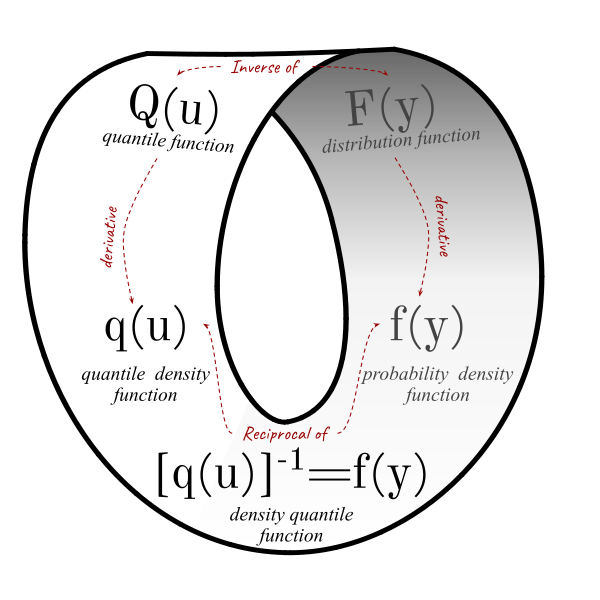
\includegraphics[width=0.4\textwidth,height=\textheight]{img/moebius-loop(1).png}

}

\caption{\label{fig-moebius-chart}Möbius strip of probability functions
\citep{perepolkin2023TenetsQuantilebasedInference}}

\end{figure}%

Although many of the distributions discussed in Section 3 have
closed-form cumulative distribution functions (CDFs) and probability
density functions (PDFs), the functional form of the quantile function
(QF) is often simpler and can be reasoned about in terms of other
quantile functions, following \emph{Gilchrist's QF transformation rules}
summarized in Table~\ref{tbl-qf-trans}. This table presents the
addition, linear combination, and multiplication rules, which involve
two quantile functions \(Q_1\) and \(Q_2\). We will refer to these three
rules as \emph{Gilchrist combinations}, as they represent valid ways to
combine quantile functions to create new quantile functions.

\begin{table}

\caption{\label{tbl-qf-trans}Gilchrist's quantile function
transformation rules \citep{gilchrist2000StatisticalModellingQuantile}}

\centering{

\centering
\begin{tabular}[t]{l>{\raggedright\arraybackslash}p{3cm}>{\raggedright\arraybackslash}p{2.5cm}>{\raggedright\arraybackslash}p{3cm}}
\toprule
Original QF & Rule & Resulting QF & Resulting variable\\
\midrule
$Q_Y(u)$ & Reflection rule & $-Q(1-u)$ & QF of -Y\\
$Q_Y(u)$ & Reciprocal rule & $1/Q(1-u)$ & QF of $1/Y$\\
$Q_1(u), Q_2(u)$ & Addition rule & $Q_1(u)+Q_2(u)$ & valid QF\\
$Q_1(u), Q_2(u)$ & Linear combination rule & $aQ_1(u)+bQ_2(u)$ & valid QF for $a,b>0$\\
$Q_1(u),Q_2(u)>0$ & Multiplication rule & $Q_1(u)Q_2(u)$ & valid QF\\
\addlinespace
$Q_Y(u)$ & Q-transformation & $T(Q_Y(u))$ & QF of $T(Y)$,\newline  $T(Y)$ non-decreasing\\
$Q_Y(u)$ & p-transformation & $Q_Y(H(u))$ & p-transformation of $Q_Y(u)$,\newline  $H(u)$ non-decreasing\\
\bottomrule
\end{tabular}

}

\end{table}%

The quantile-parameterized distributions in this paper are categorized
into two groups based on their construction method. The first group
comprises distributions that are \emph{directly} parameterized by the
quantile-probability pairs (QPPs). This group includes the Myerson
distribution \citep{myerson2005ProbabilityModelsEconomic}, and the
Johnson Quantile-Parameterized Distribution
\citep{hadlock2017JohnsonQuantileParameterizedDistributions, hadlock2019GeneralizedJohnsonQuantileParameterized}.
These distributions are constructed by reparameterizing or transforming
existing distributions, following Gilchrist rules
(Table~\ref{tbl-qf-trans}). The transformations used to construct them
are detailed in the next section.

The other group of distributions is \emph{indirectly} parameterized by
the QPPs. They require a fitting step where the quantile-probability
pairs are translated into distribution parameters, usually through
optimization or least-squares methods. This group includes the Simple
Q-Normal \citep{keelin2011QuantileParameterizedDistributions}, Metalog
\citep{keelin2016MetalogDistributions}, quantile mixtures
\citep{peng2023MixtureQuantilesEstimated}, the variant of the
Generalized Lambda Distribution (GLD) by Chalabi et al
\citep{chalabi2012FlexibleDistributionModeling}, and the
quantile-parameterized Triangular (Two-Sided Power) distribution by Kotz
and van Dorp \citep{kotz2004BetaOtherContinuous}. Each distribution's
fitting method is described in the respective subsections below.

\section{Univariate quantile-parameterized
distributions}\label{univariate-quantile-parameterized-distributions}

This section reviews various continuous univariate QPDs from the
literature. We then discuss the generalized form for these
distributions, based on the variations of these QPDs appearing in the
literature. For each distribution, we present its quantile function and
discuss the parameterization and feasibility conditions. The derivative
and inverse of each distribution can be found in Appendix A.

\subsection{Myerson distribution}\label{myerson-distribution}

One of the earliest examples of a distribution parameterized by
quantiles is the \emph{generalized log-normal} distribution defined by
the median and the upper and lower quartiles proposed by
\citep{myerson2005ProbabilityModelsEconomic}. It relies on a
transformation of the normal quantile function.

The Myerson distribution can be viewed as parameterized by three
quantile values \(\{q_1, q_2, q_3\}\), which correspond to the
cumulative probabilities \(\{\alpha, 0.5, 1-\alpha\}\). These quantiles
are symmetrical around the median and are defined by the tail parameter
\(0<\alpha<0.5\). This type of parameterization is known as the
Symmetric Percentile Triplet (SPT, \(\alpha\)-level SPT or
\(\alpha\)-SPT) and is also used in several other quantile-parameterized
distributions that we will describe below. The Myerson quantile function
is

\[
\begin{gathered}
\rho=q_3-q_2;\; 
\beta=\frac{\rho}{q_2-q_1};\;
\kappa(u)=\frac{S(u)}{S(1-\alpha)}\\
Q_Y(u \vert q_1,q_2,q_3,\alpha)=
\begin{cases}
q_2+\rho\frac{\beta^{\kappa(u)}-1}{\beta-1}, \quad &\beta \neq 1\\
q_2+\rho\kappa(u), \quad &\beta =1
\end{cases}
\end{gathered}
\]

Here, \(u\) represents the depth of the observations of the random
variable \(Y\) given the parameterizing \(\alpha\)-SPT
\(\{q_1, q_2, q_3, \alpha\}\), with \(0 < \alpha < 0.5\). The parameter
\(\rho\) is the \emph{upper p-difference}, and \(\beta\) is the ratio of
the inter-percentile ranges, known as the \emph{skewness ratio}
\citep[72]{gilchrist2000StatisticalModellingQuantile}. The \emph{kernel}
quantile function \(S(u)\) is equal to the quantile function of the
standard normal distribution, also referred to as the probit, defined as
\(S(u) = \Phi^{-1}(u)\). The formulas for the derivative and the inverse
quantile function of the Myerson QPD can be found in Appendix A.

It is important to note that while the Myerson distribution includes the
normal distribution as a special case when the skewness parameter
\(\beta = 1\), it can exhibit right-skewness or left-skewness for other
values of \(\beta\). In the symmetrical case, the range of the quantile
function is \((-\infty, \infty)\). For the right-skewed distribution
(\(\beta > 1\)), the range is
\((q_2 - \frac{\rho}{\beta - 1}, \infty)\), and for the left-skewed
distribution (\(0 < \beta < 1\)), the range is
\((-\infty, q_2 - \frac{\rho}{\beta - 1})\). The limiting case of the
skewed Myerson distribution \(\lim_{u \rightarrow 0} Q_Y(u\vert\theta)\)
for \(\beta > 1\) (and the other limit for \(0 < \beta < 1\)) possesses
some important properties that we discuss in
Section~\ref{sec-genmyerson} below.

The basic quantile function
\citep{gilchrist2000StatisticalModellingQuantile, lampasi2008AlternativeApproachMeasurement}
underlying the Myerson distribution is a simple probit,
\(S(u) = \Phi^{-1}(u)\), transformed using the exponentiation function
\(T(x) = \beta^{x}\), where \(\beta > 0\) represents the skewness ratio
\citep{gilchrist2000StatisticalModellingQuantile}. The quantile
parameterization is facilitated by \(\kappa(u)\), which takes values
\(\{-1,0,1\}\) for the three quantiles \(\{q_1, q_2, q_3\}\), such that
\(Q(\alpha) = q_1\), \(Q(0.5) = q_2\), and \(Q(1 - \alpha) = q_3\).

\subsection{Johnson Quantile-Parameterized
Distribution}\label{johnson-quantile-parameterized-distribution}

Hadlock and Bickel
\citep{hadlock2017QuantileparameterizedMethodsQuantifying} reviewed the
existing quantile-parameterized distributions and proposed the quantile
parameterization of the Johnson SU family of distributions
\citep{johnson1994ContinuousUnivariateDistributions}. In their paper,
Hadlock and Bickel
\citep{hadlock2017JohnsonQuantileParameterizedDistributions} presented
two versions of the distribution: the bounded (J-QPD-B) and the
semi-bounded (J-QPD-S), both parameterized by an SPT
\(\{q_1, q_2, q_3, \alpha\}\) and the bound(s).

The J-QPD-B distribution is obtained by applying the inverse-probit
transformation to the Johnson SU quantile function
\(Q_{SU}(u) = \xi + \lambda\sinh(\delta(S(u) + \gamma))\), where
\(\delta\) and \(\gamma\) are two shape parameters. This function is
then rescaled to the compact interval \([l_b, u_b]\). The J-QPD-B
quantile function is

\[
Q_B(u)=
\begin{cases}
l+rS^{-1}\left[Q_{SU}(u)\right], n\neq0\\
l+rS^{-1}\left[B+\kappa S(u)\right],n=0
\end{cases}
\]

where

\[
\begin{gathered}
Q_{SU}(u) = \xi + \lambda\sinh(\delta(S(u) + \gamma))\\
r=(u_b-l_b); \quad \gamma=nc; \quad \kappa=\frac{H-L}{2c}\\
S(u)=\Phi^{-1}(u); \quad c=S(1-\alpha);\\
L=S\left(\frac{q_1-l_b}{u_b-l_b}\right); \quad  B=S\left(\frac{q_2-l_b}{u_b-l_b}\right);\\
H=S\left(\frac{q_3-l_b}{u_b-l_b}\right); \quad n=\text{sgn}(L+H-2B)\\
\xi=\begin{cases}L, \quad n=1,\\
B, \quad n=0,\\
H, \quad n=-1,\end{cases}\\
\delta=\frac{1}{c}\cosh^{-1}\left(\frac{H-L}{2\min(B-L,H-B)}\right)\\
\lambda=\frac{H-L}{\sinh(2\delta c)}
\end{gathered}
\]

\begin{figure}

\centering{

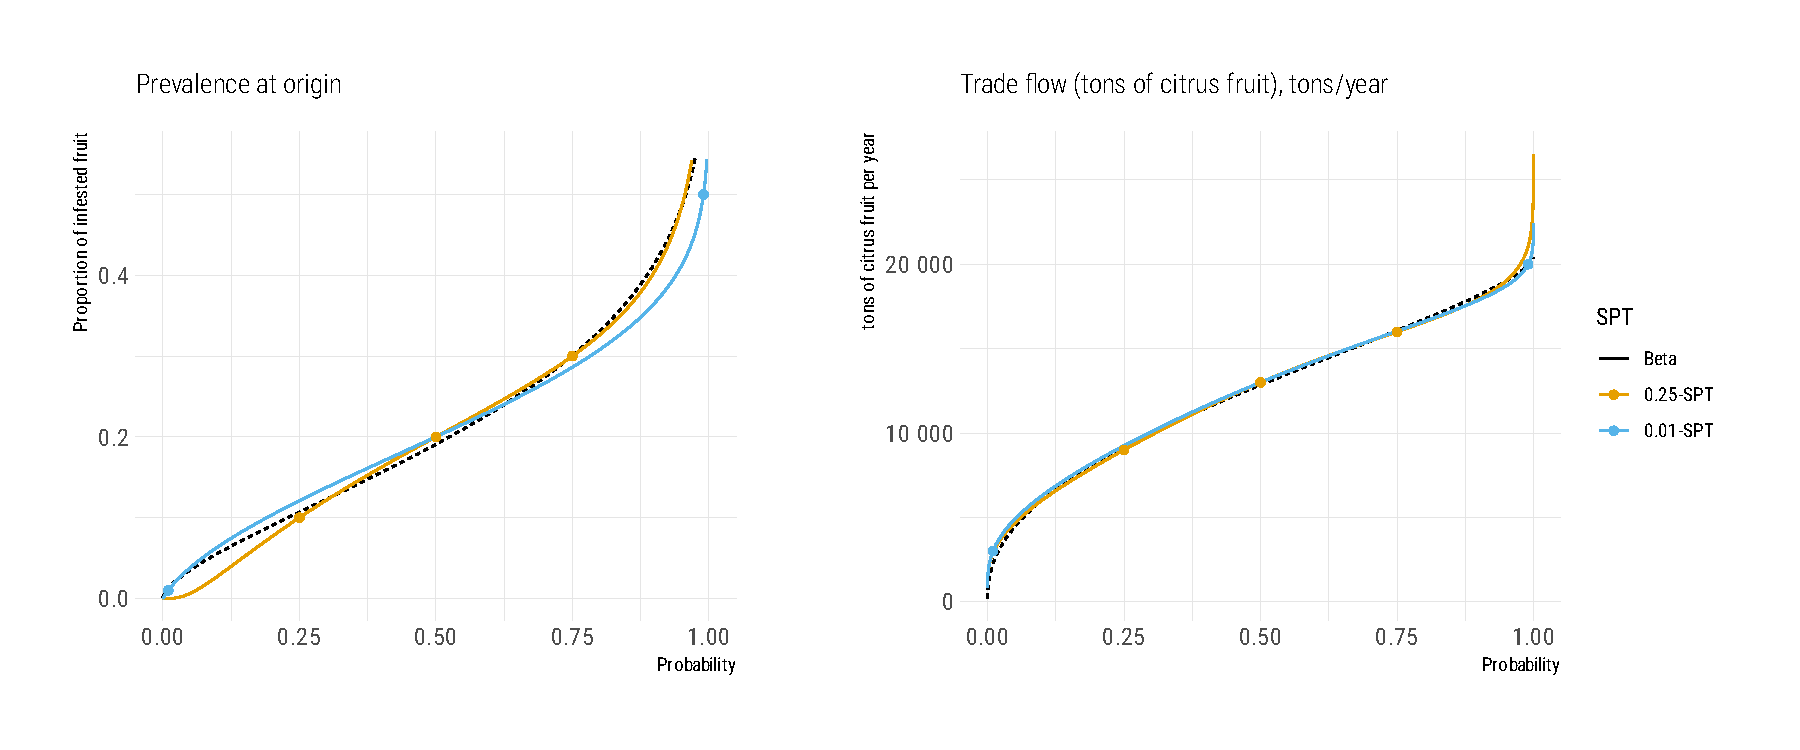
\includegraphics[width=1\textwidth,height=\textheight]{qpppp_files/figure-pdf/fig-jqpd1-1.pdf}

}

\caption{\label{fig-jqpd1}Fitted J-QPD-B (left) and J-QPD-S (right)
distribution for prevalence at origin and total trade flow,
respectively}

\end{figure}%

The left panel in Figure~\ref{fig-jqpd1} showcases the J-QPD-B quantile
function, which is parameterized using 0.25-SPT and 0.01-SPT assessments
of the proportion of fruit infested with \emph{Citripestis
sagittiferella}, as elicited by
\citep{efsa2023RiskAssessmentCitripestis}. The dashed line represents
the Beta distribution fitted by the authors. The J-QPD-B, being
parameterized by an SPT, effectively captures three of the five
parameterizing quantiles, while the Beta distribution only provides an
approximation. Finding parameters of Beta distribution requires an
optimization step.

The J-QPD-S distribution is a semi-bounded variant of the distribution
that employs exponentiated hyperbolic arcsine transformations of the
Johnson's SU quantile function
\(Q_{SUa}(u) = \xi + \lambda\sinh\left[\text{asinh}(\delta S(u)) + \text{asinh}(\delta\gamma)\right]\)
located at zero \(\xi=0\)
\citep{hadlock2017JohnsonQuantileParameterizedDistributions}

\[
\begin{gathered}
Q_S(u)=\begin{cases}
l_b+\theta\exp\left(Q_{SUa}(u)\right),n \neq 0\\
l_b+\theta\exp\left(\lambda\delta S(u)\right),n=0
\end{cases}
\end{gathered}
\]

where

\[
\begin{gathered}
Q_{SUa}(u) = \lambda\sinh\left[\text{asinh}(\delta S(u)) + \text{asinh}(\delta\gamma)\right]\\
r=(u_b-l_b); \quad \gamma=nc; \quad \kappa=\frac{H-L}{2c}\\
S(u)=\Phi^{-1}(u); \quad c=S(1-\alpha);\\
L=\ln(q_1-l_b); \quad  B=\ln(q_2-l_b);\\
H=\ln(q_3-l_b); \quad n=\text{sgn}(L+H-2B)\\
\theta=\begin{cases}
q_1-l_b, \quad n=1,\\
q_2-l_b, \quad n=0,\\
q_3-l_b, \quad n=-1,\end{cases}\\
\delta=\frac{1}{c}\sinh\left(\cosh^{-1}\left(\frac{H-L}{2\min(B-L,H-B)}\right)\right)\\
\lambda=\frac{1}{\delta c}\min(H-B, B-L)
\end{gathered}
\]

When \(n=\text{sgn}(L+H-2B)\) evaluates to zero, he resulting
distribution is a lognormal distribution with parameters
\(\mu=\ln(\theta)=\ln(q_2-l_b)\) and \(\sigma=\lambda\delta=(H-B)/c\).
This distribution has support on the interval \([l_b,\infty]\).

The right panel in Figure~\ref{fig-jqpd1} depicts the J-QPD-S quantile
function, which is parameterized using 0.25-SPT and 0.01-SPT assessments
of the total trade flow for citrus fruit imported by the EU from
Indonesia, Malaysia, Thailand, and Vietnam in tons/year
\citep{efsa2023RiskAssessmentCitripestis}.

\subsection{Generalisations of QPDs}\label{generalisations-of-qpds}

\subsubsection{Generalized Johnson Quantile-Parameterized
Distribution}\label{generalized-johnson-quantile-parameterized-distribution}

Hadlock and Bickel
\citep{hadlock2019GeneralizedJohnsonQuantileParameterized} introduced
the \emph{generalized} version of the Johnson Quantile-Parameterized
distribution system, denoted as G-QPD, by replacing the Normal
distribution in the core of the Johnson SU quantile function with the
quantile functions of the logistic and Cauchy distributions.

The generalized quantile function (QF) shares similarities with the
probit-based distribution described earlier, with \(S(u)\) defined as
the quantile function of either the logistic or Cauchy distribution.

The standard quantile function and distribution function of the logistic
distribution are given by:

\[
\begin{gathered}
S(u)= \ln\left(\frac{u}{1-u}\right)\\ 
F(y)=[\exp(-y)+1]^{-1}
\end{gathered}
\]

The standard quantile function and distribution function of the Cauchy
distribution are given by:

\[
\begin{gathered}
S(u)= \tan\left[\pi\left(u-\frac{1}{2}\right)\right];\\ F(y)=\frac{1}{ \pi}\arctan(y)+\frac{1}{2}
\end{gathered}
\]

Hadlock and Bickel
\citep{hadlock2019GeneralizedJohnsonQuantileParameterized} show that the
\emph{kernel} quantile function \(S(u)\) can be any standardized
(\(S(0.5)=0\)), symmetrical (\(s(u)=s(1-u)\)), and unbounded
(\(S(u)\in(-\infty;\infty)\)) quantile function with a smooth quantile
density \(dS(u)/du=s(u)\). The authors further showed that if \(S(u)\)
and \(S^{-1}(y)\) are expressible in closed-form, the quantile function
and distribution function of G-QPD will also be closed-form.

For the \emph{logistic} kernel, the G-QPD-S represents the generalized
log-logistic distribution, characterized by two shape parameters,
\(\lambda\) and \(\delta\). For the Cauchy kernel, the G-QPD-S
corresponds to the shifted log-Cauchy distribution
\citep{hadlock2019GeneralizedJohnsonQuantileParameterized}.

\subsubsection{Generalized Myerson distributions}\label{sec-genmyerson}

Following the approach in Hadlock and Bickel
\citep{hadlock2019GeneralizedJohnsonQuantileParameterized}, Myerson
distribution can be generalized by substituting the Normal kernel
quantile function \(S(u)=\Phi^{-1}(u)\) with an alternative symmetrical
quantile function based on the depth \(u\). Below, we discuss possible
kernels and the resulting distributions:

\textbf{Logit-Myerson distribution}. Recently Wilson et al
\citep{wilson2023ReconciliationExpertPriors} reparameterized
\emph{log-logistic distribution} in terms of a Symmetric Percentile
Triplet. Even though the authors do not recognize it as such, the
resulting quantile-parameterized distribution is a Myerson distribution
with logit kernel QF \(S(u)=\ln\left(\frac{u}{1-u}\right)\)).

There could be several reasons why one might prefer the logit function
over the probit function \citep{berkson1951WhyPreferLogits}. For
example, distribution based on logit may exhibit greater numerical
stability due to its simple closed-form quantile function, which does
not rely on numerical approximation during sampling. Logit-Myerson
distribution displays slightly heavier tails compared to the standard
(probit-based) Myerson distribution
(Figure~\ref{fig-gmyerson-qfdqf-plot1}).

\textbf{Sech-Myerson distribution}. Following the same principle adopted
by Wilson et al. \citep{wilson2023ReconciliationExpertPriors} a variant
of Myerson distribution may be created using the hyperbolic secant
quantile function:

\[
S(u)=\ln\left[\tan\left(\frac{\pi}{2}u\right)\right]
\]

The Sech-Myerson distribution possesses thicker tails than the
Logit-Myerson distribution for the same parameterizing SPT
\(\{-5,4,16, 0.25\}\) (Figure~\ref{fig-gmyerson-qfdqf-plot1}). In
Section~\ref{sec-compareqf}, we conduct a comparative analysis of
different variations of the Generalized Myerson distribution alongside
their parametric counterparts and other quantile distributions.

\begin{figure}

\centering{

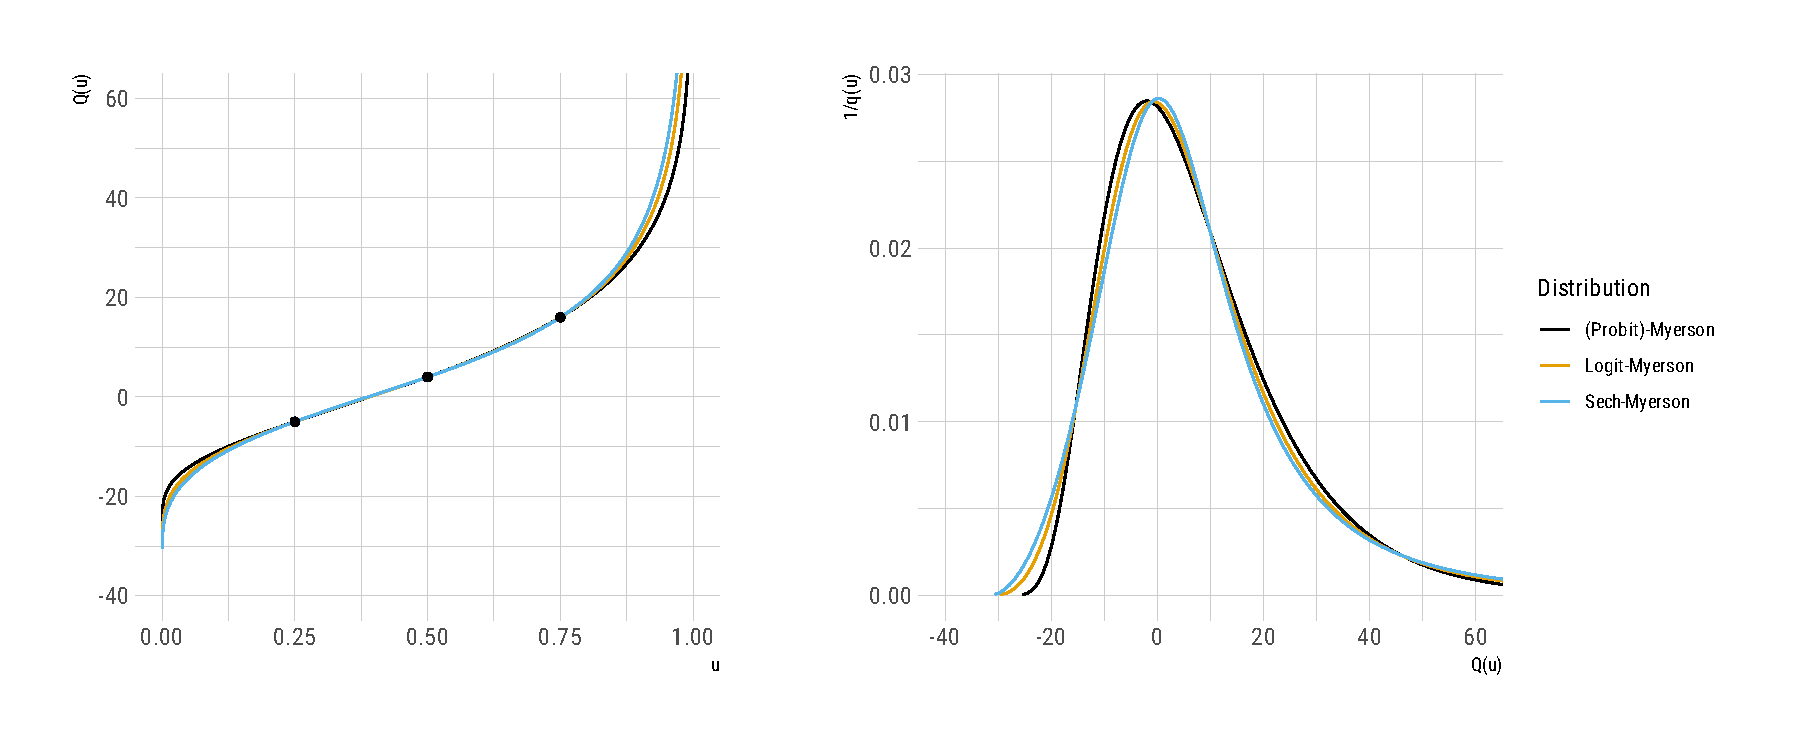
\includegraphics[width=1\textwidth,height=\textheight]{qpppp_files/figure-pdf/fig-gmyerson-qfdqf-plot1-1.pdf}

}

\caption{\label{fig-gmyerson-qfdqf-plot1}Quantile function and quantile
density of Generalized Myerson Distributions}

\end{figure}%

Theoretically, there is an infinite range of quantile function (QF)
kernels that can be utilized to generate new variations of the
Generalized Myerson distribution. These candidate kernel distributions
can even include shape parameters, as long as the resulting \(S(u)\)
remains standardized, symmetrical, and unbounded, as specified above.
For instance, it is possible to incorporate the basic QF of the Tukey
Lambda distribution \(S(u\vert\lambda)=u^\lambda-(1-u)^\lambda\) for a
fixed \(\lambda \neq 0\), or the Cauchy distribution
\(S(u)=\tan[\pi(u-0.5)]\), as employed by
\citep{hadlock2019GeneralizedJohnsonQuantileParameterized}. However, it
is important to note that not all standard quantile functions are
created equal. To illustrate the issue of unreliable kernels, let us
consider Myerson distributions based on the Cauchy and Tukey Lambda
quantile functions (for \(\lambda=-0.5\)). As can be observed in
Figure~\ref{fig-gmyerson-qfdqf-plot2}, the density of Generalized
Myerson distribution with these kernels exhibits unexpected spike near
the lower bound.

\begin{figure}

\centering{

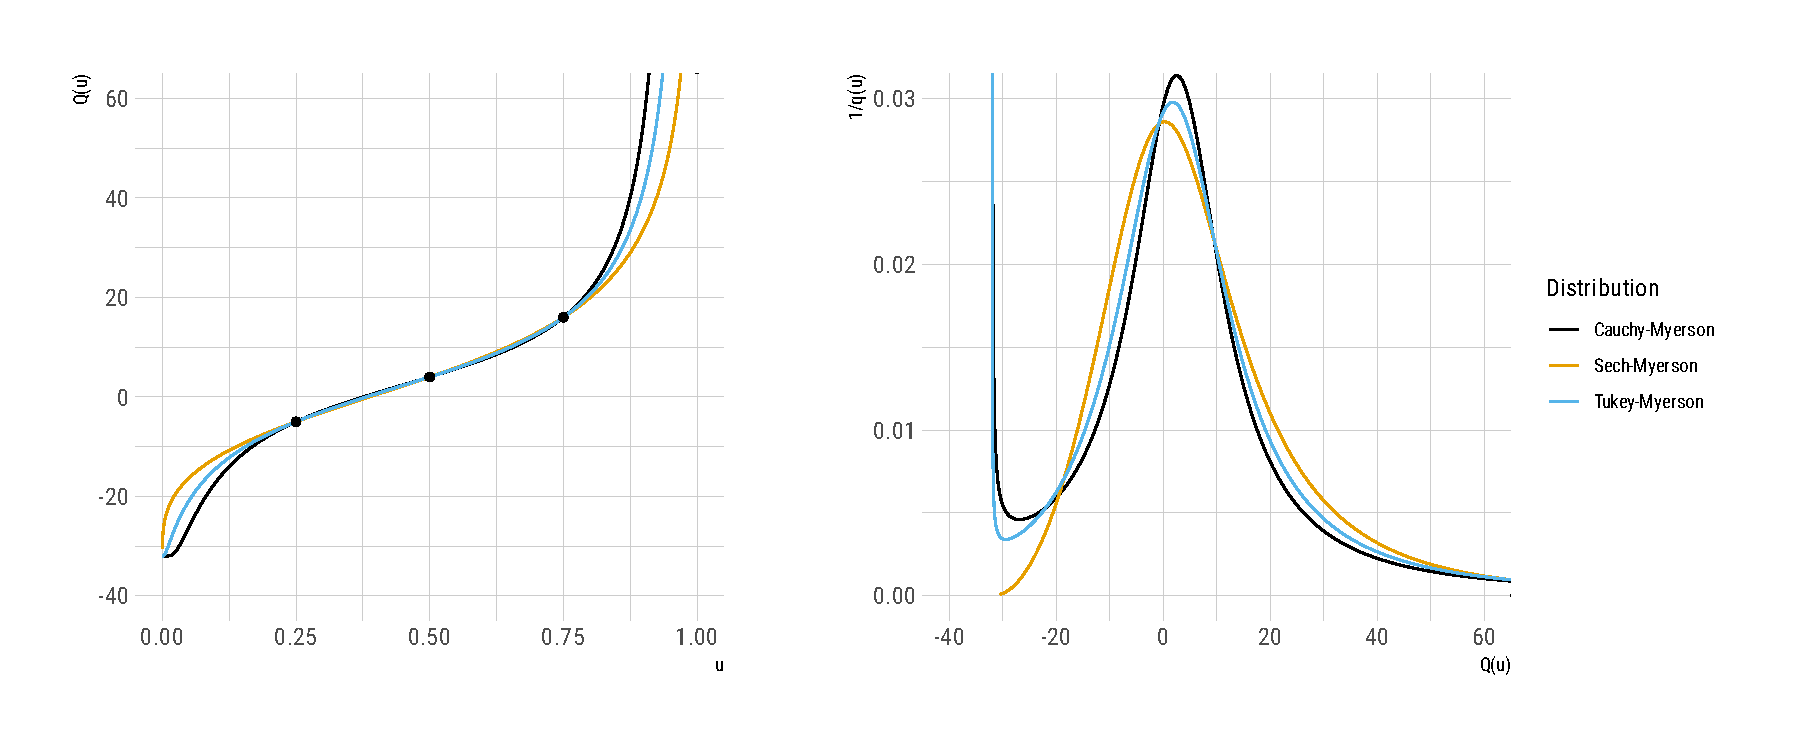
\includegraphics[width=1\textwidth,height=\textheight]{qpppp_files/figure-pdf/fig-gmyerson-qfdqf-plot2-1.pdf}

}

\caption{\label{fig-gmyerson-qfdqf-plot2}Quantile function and quantile
density of Generalized Myerson Distributions with unreliable kernels}

\end{figure}%

While all right-skewed Generalized Myerson distributions are bounded on
the left at
\(\lim_{u\rightarrow0}Q(u\vert\theta)=q_2-\rho\frac{1}{\beta-1}\)
regardless of the kernel used, the quantile density at the left limit
\(\lim_{u\rightarrow0}[q(u\vert\theta)]^{-1}\) is not independent of the
kernel. Although we can assume that \(q(0)=\infty\), the lower tail of
the density quantile function \([q(u)]^{-1}\) may exhibit a curling
effect for certain kernels, resulting in an increase in density for
lower values of \(u\). This effect is caused by the non-monotonic
behavior of the quantile convexity function \(c(u)=dq(u)/du\). This can
be easily verified by taking the second derivative of \(\beta^{S(u)}\)
for \(\beta>0\). While such kernels are mathematically valid and yield a
non-decreasing Generalized Myerson QF, we believe that they may be less
useful due to the counter-intuitive concentration of density in the
bounded tail. Consequently, we do not recommend using Cauchy or Tukey
Lambda kernels in practical applications.

\subsection{Simple Q-Normal, Metalog
distributions}\label{simple-q-normal-metalog-distributions}

An alternative system of quantile-parameterized distributions was
proposed by Keelin and Powley
\citep{keelin2011QuantileParameterizedDistributions, powley2013QuantileFunctionMethods}.
This approach relies on the finite Taylor expansion of parameters in the
standardized quantile functions. Within this framework, two
distributions were introduced: the Simple Q-Normal distribution and the
Metalog distribution.

The Simple Q-Normal (SQN) distribution was developed by expanding the
parameters in the normal quantile function. Keelin et al.~(2011) used
this method to express the parameters of the normal quantile function
\(Q(u\vert\mu,\sigma)=\mu+\sigma z(u)\) as linear functions of the depth
\(u\). Specifically, \(\mu(u)=a_1+a_4u\) and \(\sigma(u)=a_2+a_3u\),
where \(z(u)=\Phi^{-1}(u)\) denotes the standard normal quantile
function. Therefore, the quantile function of the SQN distribution can
be expressed as follows:

\begin{equation}\phantomsection\label{eq-SQNQF}{
Q(u)= a_1+a_2z(u)+a_3uz(u)+a_4u\\
}\end{equation}

where \(z(u)=\Phi^{-1}(u)\), and \(a=\{a_1,a_2,a_3, a_4\}\) represents a
vector of parameters.

Consider a quantile-probability tuple of size 4, denoted as
\(\{\mathbf{p}, \mathbf{q}\}_4\), which consists of an ordered vector of
cumulative probabilities \(\mathbf{p}=\{p_1,p_2,p_3, p_4\}\) and an
ordered vector of corresponding quantiles
\(\mathbf{q}=\{q_1,q_2,q_3, q_4\}\). Substituting these vectors into the
SQN quantile function for \(u\) and \(Q(u)\), respectively, we obtain
the following matrix equation:

\begin{equation}\phantomsection\label{eq-sqn-matrix}{
\mathbf{q}=\mathbb Pa
}\end{equation}

where

\[
\begin{gathered}
\mathbb P=\begin{bmatrix} 1 & z(p_1) & p_1z(p_1) & p_1\\
                1 & z(p_2) & p_2z(p_2) & p_2\\
                1 & z(p_3) & p_3z(p_3) & p_3\\
                1 & z(p_4) & p_4z(p_4) & p_4\end{bmatrix}
\end{gathered}
\]

and \(a=\{a_1, a_2, a_3, a_4\}\) represents the parameter vector of the
SQN distribution.

The parameter vector \(a\) can be obtained by solving the matrix
Equation~\ref{eq-sqn-matrix}, given the 4-element quantile-probability
tuple \(\{\mathbf{p}, \mathbf{q}\}_4\)
\citep{keelin2011QuantileParameterizedDistributions, perepolkin2021HybridElicitationIndirect}.

The same approach was later employed by
\citep{keelin2016MetalogDistributions} in creating the metalog
(meta-logistic) distribution. Starting with the quantile function of the
logistic distribution \(Q(u\vert\mu,s)=\mu+s\text{logit}(u)\), where
\(\mu\) corresponds to the mean and \(s\) is proportional to the
standard deviation \(\sigma=s\pi/\sqrt3\),
\citep{keelin2016MetalogDistributions} expanded the parameters \(\mu\)
and \(s\) using a finite Taylor series centered at 0.5. Specifically,
\(\mu(u)=a_1+a_4\check{u}+a_5\check{u}^2+\dots\) and
\(s(u)=a_2+a_3\check{u}+a_6\check{u}^2+\dots\), where
\(\check{u}=u-0.5\) and \(a_i, \; i = \{1,2,\dots,n\}\) are real
constants.

Therefore, the metalog quantile function is:

\[
\begin{gathered}
Q(u)= a_1+a_2\text{logit}(u)+a_3\check{u}\text{logit}(u)+\\
a_4\check{u}+a_5\check{u}^2\cdots,
\end{gathered}
\]

Given a QPT of size \(m\) denoted by \(\{\mathbf{p}, \mathbf{q}\}_m\),
where \(\mathbf{p}\) and \(\mathbf{q}\) are ordered vectors of
cumulative probabilities and corresponding quantiles, respectively, the
vector of coefficients \(\mathbf{a}={a_1,\dots,a_m}\) can be determined
by solving the matrix equation \(\mathbf{q}=\mathbb{P}\mathbf{a}\),
where \(\mathbf{p}\), \(\mathbf{q}\), and \(\mathbf{a}\) are column
vectors, and \(\mathbb{P}\) is an \(m \times n\) matrix:

\begin{equation}\phantomsection\label{eq-metalogPMatrixeq}{
\begin{gathered}
\mathbb{P} = \left[\begin{array}{lllll}
1  &\text{logit}(p_1) &\check{p}_1\text{logit}(p_1) &\check{p}_1 &\cdots\\
1  &\text{logit}(p_2) &\check{p}_2\text{logit}(p_2) &\check{p}_2 &\cdots\\
   &                  &\vdots\\
1  &\text{logit}(p_m) &\check{p}_m\text{logit}(p_m) &\check{p}_m &\cdots
\end{array}\right]
\end{gathered}
}\end{equation}

The vector of coefficients \(\mathbf{a}\) can be determined as
\(\mathbf{a}=[\mathbb{P}^{T}\mathbb{P}]^{-1}\mathbb{P}^{T}\mathbf{q}\).
If \(\mathbb{P}\) is a square matrix, meaning the number of terms \(n\)
is equal to the size of the parameterizing QPT \(m\), the equation can
be further simplified to \(\mathbf{a}=\mathbb{P}^{-1}\mathbf{q}\).
Metalog is said to be \emph{approximated} when the number of
quantile-probability pairs used for parameterization exceeds the number
of terms in the metalog QF
\citep{keelin2016MetalogDistributions, perepolkin2021HybridElicitationIndirect}.

The SQN and Metalog distributions are families of extended distributions
that, in theory, can have an arbitrary number of terms. Keelin
\citep{keelin2016MetalogDistributions} demonstrated the flexibility of
the metalog distribution and its ability to approximate arbitrarily
complex probability density functions with high precision, given enough
terms in the metalog specification. In practice, 10-15 terms are
sufficient to approximate the distributional shapes of virtually any
complexity \citep{keelin2021MetalogDistributionsVirtually}. Keelin
\citep{keelin2016MetalogDistributions} introduced the bounded
logit-metalog, the semi-bounded log-metalog, and a special case of a
3-term metalog parameterized by \(\alpha\)-SPT (SPT-metalog).

However, not all combinations of parameters \(\mathbf{a}\) in metalog
and SQN distributions result in a feasible (non-decreasing) quantile
function. For an arbitrary \(\mathbf{a}\)-vector, feasibility must be
checked \citep{keelin2011QuantileParameterizedDistributions}. In the
case of 3-term metalogs, the feasibility conditions are straightforward
\citep{keelin2016MetalogDistributions}. But as the number of terms
increases, such conditions become increasingly complex
\citep{keelin2017MetalogDistributionsFeasibility}. Having to deal with
such feasibility requirements stands in contrast with QF's that are
constructed using Gilchrist rules Table~\ref{tbl-qf-trans}, which
guarantee feasibility.

\subsection{Quantile mixtures}\label{quantile-mixtures}

Recently \citep{peng2023MixtureQuantilesEstimated} proposed a novel
framework for extended quantile-parameterized distributions based on
quantile mixtures (not to be confused with CDF/PDF mixtures,
\citep[107]{gilchrist2000StatisticalModellingQuantile}). They introduced
a formulation in which a QPD quantile function is expressed as a linear
combination of \(I\) standardized quantile functions, following
Gilchrist's \emph{linear combination rule} (Table~\ref{tbl-qf-trans}):

\[
G(u\vert\theta)=\sum_{i=0}^I\theta_iQ_i(u)
\]

Here, \(Q_i(u)\) represent basis quantile functions for the random
variable \(Y\) with \(Q_0(u)=1\), and
\(\pmb\theta=\{\theta_0,\theta_1,\dots,\theta_I\}\) is a non-negative
parameter vector that determines the contribution of each QF component
in the quantile mixture. To compute the coefficients \(\pmb\theta\), the
system of equations is solved

\[
\mathbf q=\mathbb Q \pmb\theta+\pmb\epsilon
\]

where \(\mathbf{q}=\{q_1,q_2,\dots, q_j\}\) is an ordered vector of
\(J\) parameterizing quantiles, corresponding to an ordered vector of
cumulative probabilities \(\mathbf{p}=\{p_1,p_2,\dots, p_j\}\),
\(\pmb\theta\) is a non-negative vector of \(I+1\) parameters,
\(\pmb\epsilon\) is a \(J\)-size vector of errors to be minimized, and
\(\mathbb Q\) is a \(J\times(I+1)\) matrix of regression factors

\[
\begin{gathered}
\mathbb{Q} = \left[\begin{array}{lllll}
1  &Q_1(p_1) &Q_2(p_1) &\cdots &Q_I(p_1)\\
1  &Q_1(p_2) &Q_2(p_2) &\cdots &Q_I(p_2)\\
   &\vdots   &\vdots   &\ddots \\
1  &Q_1(p_J) &Q_2(p_J) &\cdots &Q_I(p_J)
\end{array}\right]
\end{gathered}
\]

By ensuring non-negativity of weights (\(\theta_i\geq0\)), the solution
guarantees a proper non-decreasing quantile function. To estimate the
values of the vector \(\pmb\theta\in\Theta\), the authors suggest using
constrained weighted least squares regression with optional
regularization. The authors demonstrated that the estimator
\(\widehat{\pmb\theta}=\underset{\pmb\theta\in\Theta}{\text{argmin}} \left(\frac{1}{J}\sum_{j=1}^Jw_j\mathcal{E}_q(y_j-Q_j\pmb\theta)\right)^{\frac{1}{q}}\),
\(\mathcal{E}_q(x)=\lvert x \rvert^q\), \(w_j>0\), is asymptotically a
q-Wasserstein distance estimator, which converges in distribution to a
Normal distribution. The paper \citep{peng2023MixtureQuantilesEstimated}
includes the application of the quantile mixture model using a large
number of asymmetric t-distributions, and a quantile mixture of
Generalized Beta II distributions.

The quantile mixtures method of creating new QPDs guarantees feasibility
by construction, while affording nearly infinite flexibility, provided
that the component quantile functions are selected from a wide set of
distributions of varying shapes. Besides, a QPD constructed as a linear
combination of QFs is guaranteed to be unimodal, unless one of the
component in the mixture is multimodal \citep[see][ for
examples]{gilchrist2000StatisticalModellingQuantile}. In addition, the
method proposed by \citep{peng2023MixtureQuantilesEstimated} offers an
advantage of resulting in closed-form quantile function and quantile
density function, provided that each of the components can be expressed
analytically. Unfortunately, neither asymmetric t-distribution nor
Generalized Beta II distribution, used by the authors, has a closed-form
QF. However, one can construct a highly flexible quantile function using
Gilchrist rules (Table~\ref{tbl-qf-trans}) or use one of the existing
well-studied QFs discussed in the literature. In
Section~\ref{sec-qmexample}, we provide an example of using a quantile
mixture of diversely-shaped quantile functions to construct a bespoke
highly flexible QPD.

\subsection{Other distributions}\label{other-distributions}

\subsubsection{Triangular and Two-Sided Power
distributions}\label{triangular-and-two-sided-power-distributions}

Several other distributions with at least some parameters mapped to
quantiles were proposed, including the reparameterization of the
Generalized Lambda Distribution by
\citep{chalabi2012FlexibleDistributionModeling} and the
quantile-parameterized triangular (two-sided power) distribution by
\citep{kotz2004BetaOtherContinuous}.

Kotz and van Dorp \citep{kotz2004BetaOtherContinuous} describe the
quantile-parameterized version of the triangular distribution
\citep{johnson1997TriangularDistributionProxy}. This bounded
distribution is widely used in the finance and insurance industry and is
popularized by the @Risk software package, developed by Palisade
\citep{palisadecorporation2009GuideUsingRISK}. The triangular
distribution is parameterized by the two quantiles \(q_{a}\) and
\(q_{b}\), and the mode \(m\), subject to the constraint that
\(a\leq q_a\leq m\leq q_b\leq b\), where \(a\) and \(b\) represent the
lower and upper bounds, respectively. The standard quantile function for
the triangular distribution is expressed in terms of the bounds \(a\),
\(b\), and the mode \(m\).

\[
\begin{gathered}
Q(u)=\begin{cases}
a+\sqrt{ud_ld}, \; \text{for } 0\leq u \leq\frac{d_l}{d}\\
b-\sqrt{(1-u)d_ud}, \; \text{otherwise}
\end{cases}
\end{gathered}
\]

where \(d=b-a;\; d_l=m-a;\; d_u=b-m\).

In \citep{kotz2004BetaOtherContinuous} the authors show that given the
two parameterizing quantile-probability pairs \(\{q_a,p_a\}\) and
\(\{q_b,p_b\}\) and the mode value \(m\), there exists a unique value of
depth \(p_a<p<p_b\) corresponding to the root of the function

\[
g(p)=\frac{(m-q_a)(1-\tau_b)}{(q_b-m)(1-\tau_a)+(m-q_a)(1-\tau_b)}-p
\]

where \(\tau_b=\sqrt{\frac{1-p_b}{1-p}}\),
\(\tau_a=\sqrt{\frac{p_a}{p}}\).

The root value \(p\in (p_a,p_b)\) of the function \(g(p)\) can be found
using any of the bracketing root-finding algorithms
\citep{perepolkin2023TenetsQuantilebasedInference}. It can then be
substituted into the following expressions to find the lower \(a\) and
upper \(b\) limit parameters of the triangular distribution:

\[
\begin{gathered}
a(p) \equiv \frac{q_a-m\tau_a}{1-\tau_a}, \quad a(p)<q_a\\
b(p) \equiv \frac{q_b-m\tau_b}{1-\tau_b}, \quad b(p)>q_b
\end{gathered}
\] where \(\tau_b=\sqrt{\frac{1-p_b}{1-p}}\),
and\(\tau_a=\sqrt{\frac{p_a}{p}}\).

The book \citep{kotz2004BetaOtherContinuous} provides an algorithm for
fitting a four-parameter generalization of the triangular distribution
called the Two-Sided Power Distribution (TSP), using three
quantile-probability pairs and a mode value. For more information on
fitting the Quantile-Parameterized TSP Distribution by quantiles, refer
to Section 4.3.3 of \citep{kotz2004BetaOtherContinuous}.

\subsubsection{Generalized Lambda Distribution}\label{sec-gld}

Chalabi, Scott and Würtz (CSW)
\citep{chalabi2012FlexibleDistributionModeling} proposed an
asymmetry-steepness reparameterization of the Generalized Lambda
Distribution (GLD) \citep{freimer1988StudyGeneralizedTukey} with four
parameters. This reparameterization involves mapping the location to the
median and the scale to the interquartile range (IQR), which corresponds
to the first and second robust moments
\citep{kim2004MoreRobustEstimation, moors1988QuantileAlternativeKurtosis}.

The reparameterized Generalized Lambda Distribution (CSW GLD) has a
quantile function given by

\[
Q(u\vert\tilde\mu,\tilde\sigma,\chi,\xi)=\tilde\mu+\tilde\sigma\frac{S\left(u\vert\chi,\xi\right)-S\left(\frac{1}{2}\vert\chi,\xi\right)}{S\left(\frac{3}{4}\vert\chi,\xi\right)-S\left(\frac{1}{4}\vert\chi,\xi\right)}
\]

where \(\tilde\mu,\tilde\sigma,\chi,\xi\) represent the location, scale,
asymmetry, and steepness parameters, respectively. The specific form of
the basic function \(S(u)\) depends on the values of the parameters
\(\chi\) and \(\xi\)

\[
\begin{gathered}
S(u\vert\chi,\xi)=\\
\begin{cases}
\begin{aligned}
&\ln(u)-\ln(\bar{u}),  \; \text{if }\chi=0,\xi=0.5&\\
&\ln(u)-\frac{\bar{u}^{2\alpha}-1}{2\alpha}, \; \text{if }\chi\neq0,\xi=\frac{1}{2}(1+\chi)&\\
&\frac{u^{2\beta}-1}{2\beta}-\ln(\bar{u}), \; \text{if }\chi\neq0,\xi=\frac{1}{2}(1-\chi)&\\
&\frac{u^{\alpha+\beta}-1}{\alpha+\beta}-\frac{\bar{u}^{\alpha-\beta}-1}{\alpha-\beta}, \; \text{otherwise}
\end{aligned}
\end{cases}
\end{gathered}
\]

where \(\alpha=0.5\frac{0.5-\xi}{\sqrt{\xi(1-\xi)}}\) and
\(\beta=0.5\frac{\chi}{\sqrt{1-\chi^2}}\). The bounds of the
distribution are given by

\[
\begin{gathered}
S(0\vert\chi,\xi)=\begin{cases}
\begin{aligned}
&-\frac{1}{\alpha+\beta},\quad &\text{if }\xi<\frac{1}{2}(1+\chi)\\
&-\infty, \quad &\text{otherwise}
\end{aligned}
\end{cases}\\
S(1\vert\chi,\xi)=\begin{cases}
\begin{aligned}
&\frac{1}{\alpha-\beta},\quad &\text{if }\xi<\frac{1}{2}(1-\chi)\\
&\infty, \quad &\text{otherwise}
\end{aligned}
\end{cases}
\end{gathered}
\]

The CSW GLD can have unbounded, bounded, and semi-bounded support,
accommodating a wide range of shapes, including unimodal, monotone,
U-shaped, and S-shaped densities
\citep{chalabi2012FlexibleDistributionModeling}. Although the CSW GLD is
not strictly parameterized by quantiles, the mapping of the location and
scale parameters to the median and IQR makes it a suitable candidate for
expert-informed distribution specification.

Several specialized methods have been developed for fitting the GLD to
samples \citep{karian2003ComparisonGLDFitting}. The parameterization of
the CSW GLD simplifies the fitting process because two of the four
parameters can be directly calculated from the sample: the location
parameter is equal to the sample median, and the scale parameter is
equal to the interquartile range. The remaining parameters can be
estimated using various methods, including robust moment matching,
quantile matching, trimmed L-moments, distributional least
squares/absolutes, as well as maximum likelihood estimation
\citep{chalabi2012FlexibleDistributionModeling, gilchrist2000StatisticalModellingQuantile}.
The range of feasible values for the steepness and asymmetry parameters
can be further reduced with the shape conditions specified in Section
3.5 of \citep{chalabi2012FlexibleDistributionModeling}.

Recently, \citep{dedduwakumara2021EfficientEstimatorParameters} proposed
a new method of matching the shape of the GLD distribution to data using
the probability density quantile (pdQ) function
\citep{staudte2017ShapesThingsCome}. For the quantile function
\(Q(v), \; v\in [0,1]\) and the corresponding density quantile function
\(f(Q(v))=[q(v)]^{-1}\), the pdQ is defined as

\[
f^*(v)=\frac{f(Q(v))}{E\left[f(Q(v))\right]}
\]

The probability density quantile function is defined on the unit square
and is independent of the location and scale parameters.

Since integrating the GLD density quantile function is difficult,
\citep[Section 2.2]{staudte2017ShapesThingsCome}, proposed using the
kernel density method to estimate the empirical QDF and, thus, an
empirical pdQ for samples from continuous distributions. Fitting the CSW
GLD to a sample can be reduced to finding the asymmetry and steepness
parameters that minimize

\[
\underset{\chi,\xi}{\text{argmin}}\int_0^1\left[f^*(v, \chi, \xi)-f_{e}^*(v)\right]^2du
\]

where \(f^*(v,\chi,\xi)\) is the pdQ of the CSW GLD, and \(f^*_e(v)\) is
the empirical pdQ of the sample. The authors
\citep{dedduwakumara2021EfficientEstimatorParameters} suggest
approximating the integral by a discrete set of depths \(v\), replacing
the integral with a sum.

\subsection{Example}\label{sec-qmexample}

As an illustration of a faithful approximation of a large number of
quantile-probability pairs by QPD, we take 4000 posterior samples (4
chains of 1000 samples each) of one of the random intercepts in the
Eight Schools example model included in the \texttt{cmdstanr} package
\citep{gabry2022CmdstanrInterfaceCmdStan} in R. The Eight Schools
problem \citep{rubin1981EstimationParallelRandomized} measuring the
effectiveness of SAT coaching program in 8 US schools is often used as
an example model in introductory classes on Bayesian Statistics. In
\texttt{cmdstanr} it is modeled using a hierarchical Bayesian model with
normal priors for each of the 8 random intercepts \texttt{theta}.
However, due to the low number of posterior samples and the
heterogeneity in the data, the marginal posterior distributions of the
intercept parameters \texttt{theta} deviate from the Gaussian shape in
various ways (Figure~\ref{fig-school-thetas}).

An empirical distribution of posterior samples from a Bayesian model can
be viewed as a large number of quantile-probability pairs. Although it
is unlikely that such number of quantile-probability pairs could ever be
elicitable from an expert (in our case 4000), it could still be of
interest to approximate such marginal posterior distribution with a
highly flexible quantile function, e.g.~for the purpose of posterior
passing
\citep{brand2019CumulativeScienceBayesian, pritsker2021ComparingBayesianPosterior}.
Closed-form QF expression for the posterior margins would allow reusing
it as a prior in a similar model at a later stage. We discuss
multivariate extension of this idea in
Section~\ref{sec-multivariateqpd}.

\begin{figure}

\centering{

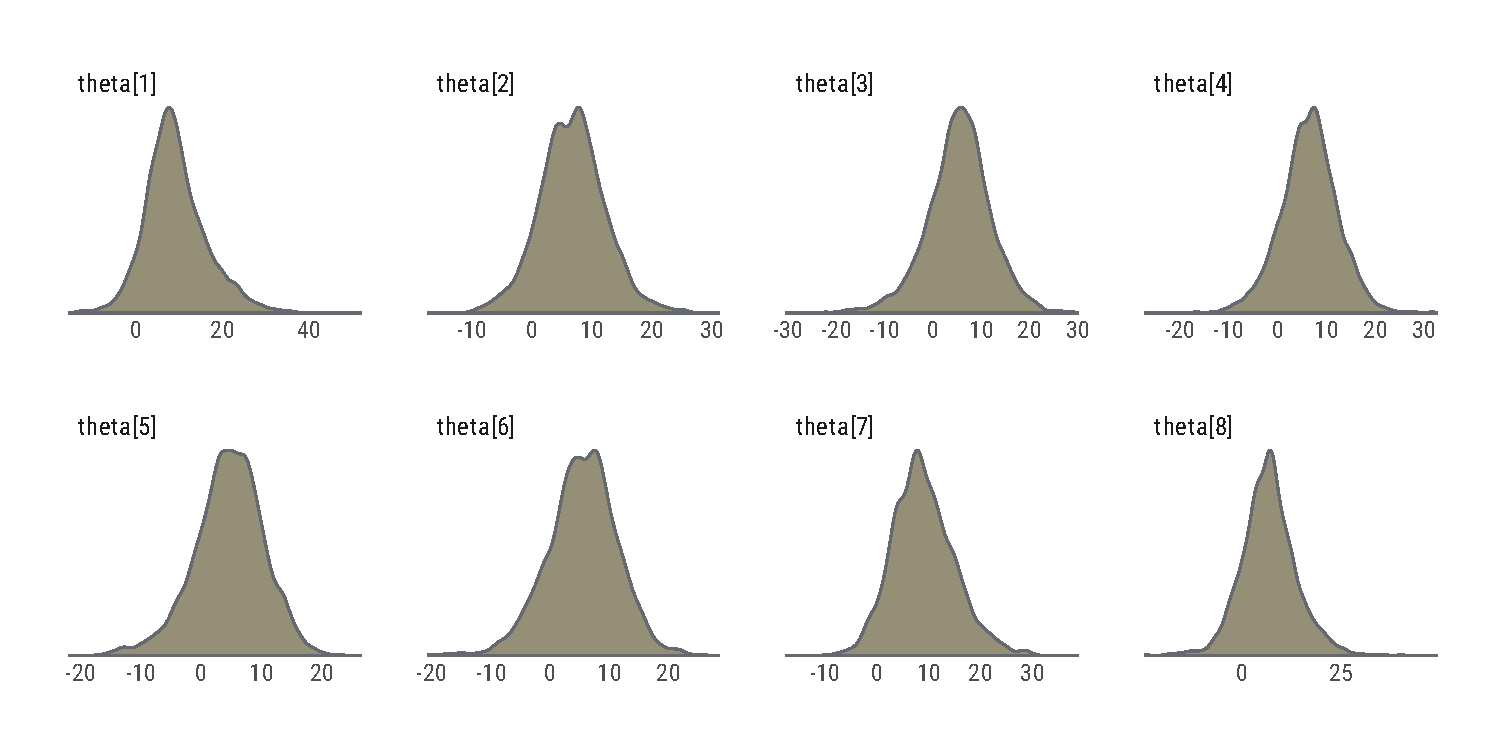
\includegraphics[width=1\textwidth,height=\textheight]{qpppp_files/figure-pdf/fig-school-thetas-1.pdf}

}

\caption{\label{fig-school-thetas}Posterior distributions of random
interecept parameters \texttt{theta} in the Eight Schools example model
\citep{gabry2022CmdstanrInterfaceCmdStan}}

\end{figure}%

Figure~\ref{fig-fitted-qm} shows a QPD approximation of the marginal
distribution of \texttt{theta{[}5{]}} using a quantile mixture of
standardized (centered at zero and with the scale parameter set to one)
\citet{chalabi2012FlexibleDistributionModeling} Generalized Lambda
Distributions (CSW GLD). In order to ensure the diversity of mixture
components we generated 400 independent uniformly distributed pairs of
the two shape parameters for GLD components using
\citet{hubbard2019MultiDimensionalCounterBasedPseudo} pseudo random
number generator.

We constructed the matrix \(\mathbb Q\) above following the method
outlined by \citet{peng2023MixtureQuantilesEstimated} and used
Lawson-Hanson non-negative least squares algorithm (implemented in
\texttt{nnls} package \citep{mullen2023NnlsLawsonhansonAlgorithm} in R)
to find the weights for each of the mixture components. The non-zero
elements are shows in Figure~\ref{fig-gld-comp} along with the weights
(which become the scale parameters of the quantile mixture components).

\begin{figure}

\centering{

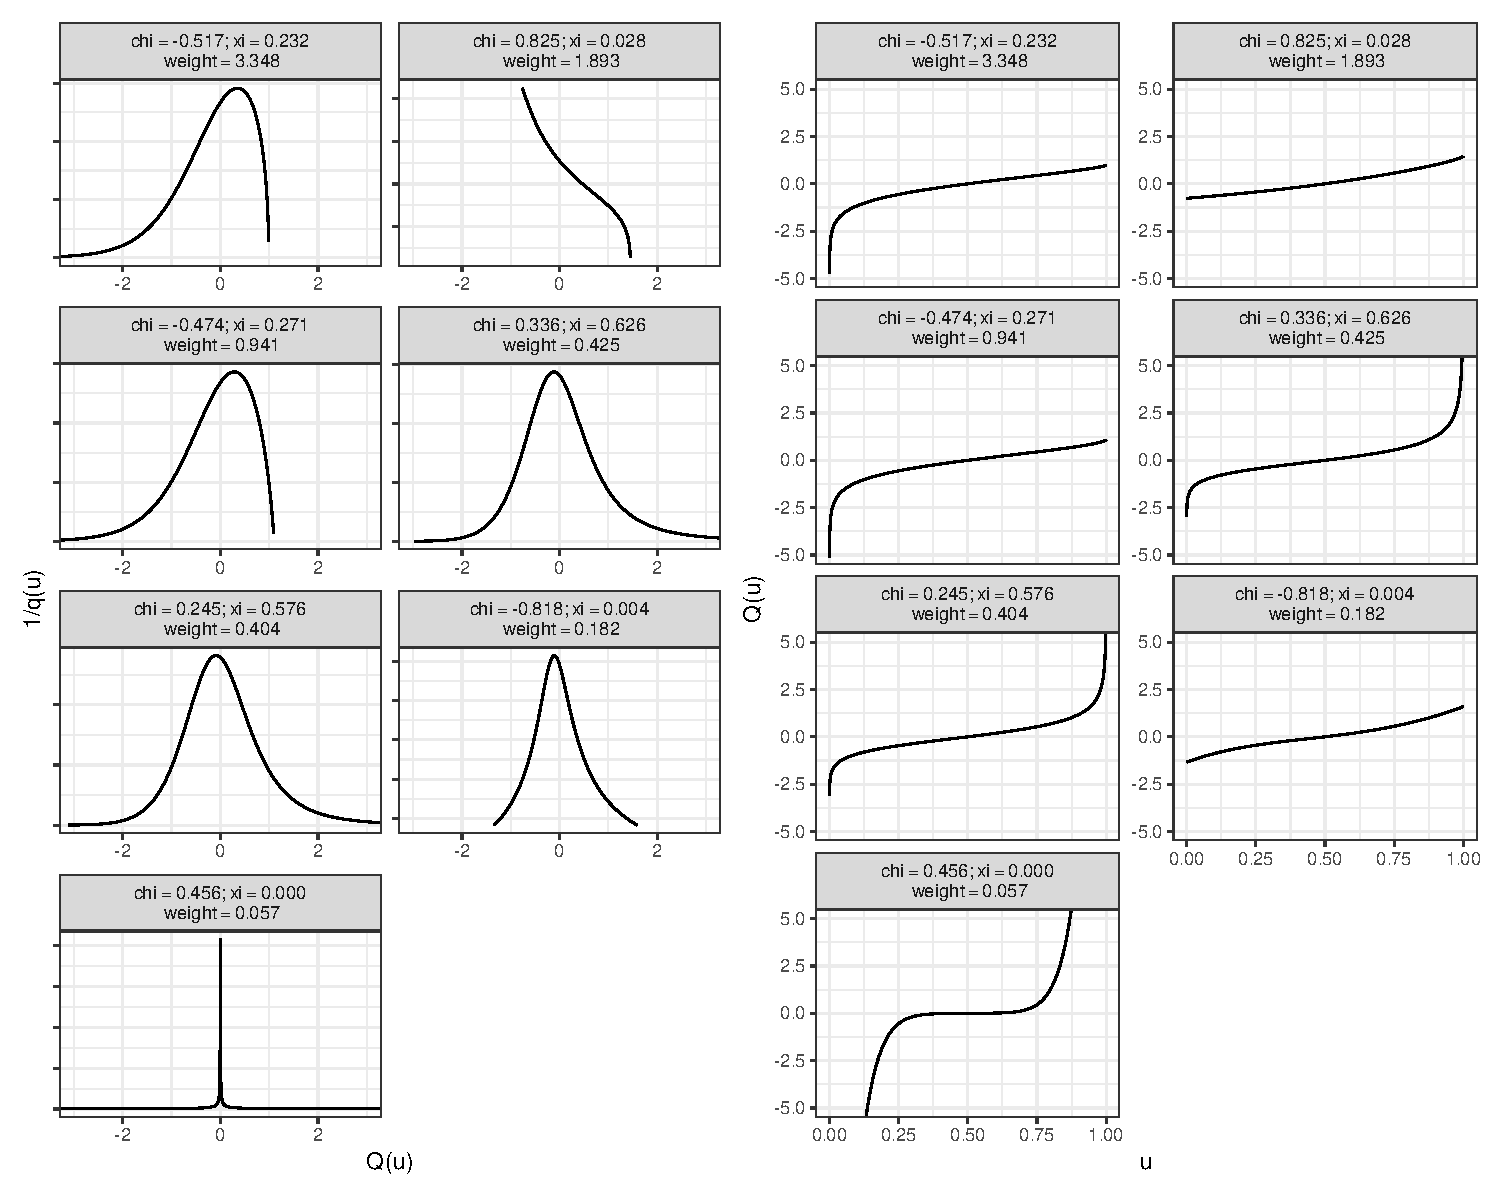
\includegraphics[width=1\textwidth,height=\textheight]{qpppp_files/figure-pdf/fig-gld-comp-1.pdf}

}

\caption{\label{fig-gld-comp}Density functions and quantile functions of
GLD components in approximating quantile mixture}

\end{figure}%

\begin{figure}

\centering{

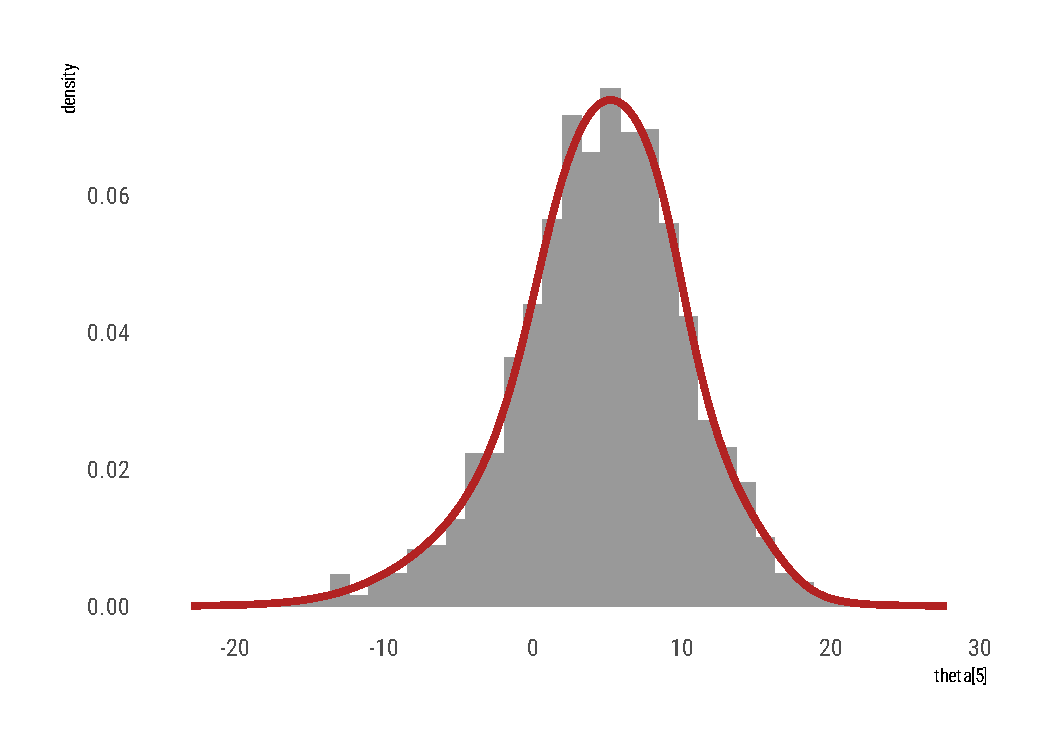
\includegraphics[width=0.8\textwidth,height=\textheight]{qpppp_files/figure-pdf/fig-fitted-qm-1.pdf}

}

\caption{\label{fig-fitted-qm}Distribution of posterior samples
approximated by the quantile mixture}

\end{figure}%

Figure~\ref{fig-fitted-qm} shows the histogram of 4000 parameter values
for \texttt{theta{[}5{]}} along with the approximation using the
quantile mixture with the components shown in Figure~\ref{fig-gld-comp}.
The resulting mixture is a linear combination of GLD quantile functions
with a closed form QF and DQF, which makes it possible to reuse this
distribution as a quantile-based prior in a Bayesian model
\citep{perepolkin2023TenetsQuantilebasedInference}.

\subsection{Choosing quantile-parameterized
distribution}\label{sec-compareqf}

A common approach to assess the properties of probability distributions
is through central moments, denoted by \(\mu_k=\mathbb{E}[(Y-\mu)^k]\),
where \(\mu\) represents the expected value of \(Y\). Karl Pearson
introduced a classification system for distributions using moment ratios
associated with skewness and kurtosis
\citep{fiori2009KarlPearsonOrigin}:

\[
\beta_1=\frac{\mu_3^2}{\mu_2^3},\quad \beta_2=\frac{\mu_4}{\mu_2^2}
\]

While computing moments using the quantile function is straightforward
(the \(n\)-th raw moment is \(\mu_k=\int_0^1Q(u)^kdu\)), it may not be
possible to calculate higher-order moments for certain distributions.

Alternatively, robust alternatives to moments can be utilized, such as
the sample median \(\mu_r\), the interquartile range \(\sigma_r\), the
quartile-based robust coefficient of skewness \(s_r\)
\citep{kim2004MoreRobustEstimation}, also known as Bowley's skewness
\citep{bowley1920ElementsStatistics} or Galton's skewness
\citep{gilchrist2000StatisticalModellingQuantile}, and the octile-based
robust coefficient of kurtosis \(\kappa_r\), also known as Moors'
kurtosis \citep{moors1988QuantileAlternativeKurtosis}.

\[
\begin{aligned}
&\mu_r=Q(1/2)\\
&\sigma_r=Q(3/4)-Q(1/4)\\
&s_r=\frac{Q(3/4)+Q(1/4)-2Q(1/2)}{\sigma_r}\\
&\kappa_r=\frac{Q(7/8)-Q(5/8)+Q(3/8)-Q(1/8)}{\sigma_r}
\end{aligned}
\]

\citep{kim2004MoreRobustEstimation, arachchige2022RobustAnalogsCoefficient}
have proposed to standardize robust moments to facilitate their
comparison with the corresponding robust moments of the standard normal
distribution.
\citep{groeneveld1998ClassQuantileMeasures, jones2011SkewnessInvariantMeasuresKurtosis}
have introduced generalizations of robust moments to other quantiles.

Unlike moments, quantiles are always well defined, and since QPDs are
parameterized by quantile-probability pairs, quantile-based robust
moments can sometimes be directly computed from the parameters. For
instance, if the basic quantile function \(S(u)\) in
\(Q(u)=\mu+\sigma S(u)\) is standardized (such that \(S(0.5)=0\)), where
\(\mu\) and \(\sigma\) are the location and scale parameters of \(Q(u)\)
respectively, then \(\mu_r=\mu\). Moreover, \(\sigma_r\) is always
independent of location, and \(s_r\) and \(\kappa_r\) are independent of
both location and scale.

Figure~\ref{fig-unbounded}, Figure~\ref{fig-semibounded}, and
Figure~\ref{fig-bounded} resemble the Cullen and Frey
\citep{cullen1999ProbabilisticTechniquesExposure} plots (Pearson plots),
but instead of using central moments, they employ quartile/octile-based
robust metrics of skewness \(s_r\) and kurtosis \(\kappa_r\) to compare
the quantile-parameterized distributions to some of their parametric
counterparts.

In these plots, Metalog3 and Metalog4 refer to 3- and 4-term metalog
distributions, respectively, and GLDcsw refers to Chalabi et al
\citep{chalabi2012FlexibleDistributionModeling} parameterization of GLD.
As can be seen in Figure~\ref{fig-unbounded}, all generalizations of
Myerson distributions have higher robust kurtosis for the same robust
skewness. Additionally, GLD CSW is more flexible than the unbounded
4-term metalog. The \emph{log}-transformed metalog distribution appears
to be the best among the semi-bounded distributions
(Figure~\ref{fig-semibounded}). Furthermore, the flexibility of the
bounded J-QPD-B is at least as good as that of the Beta and Kumaraswamy
distributions (Figure~\ref{fig-bounded}).

\begin{figure}

\centering{

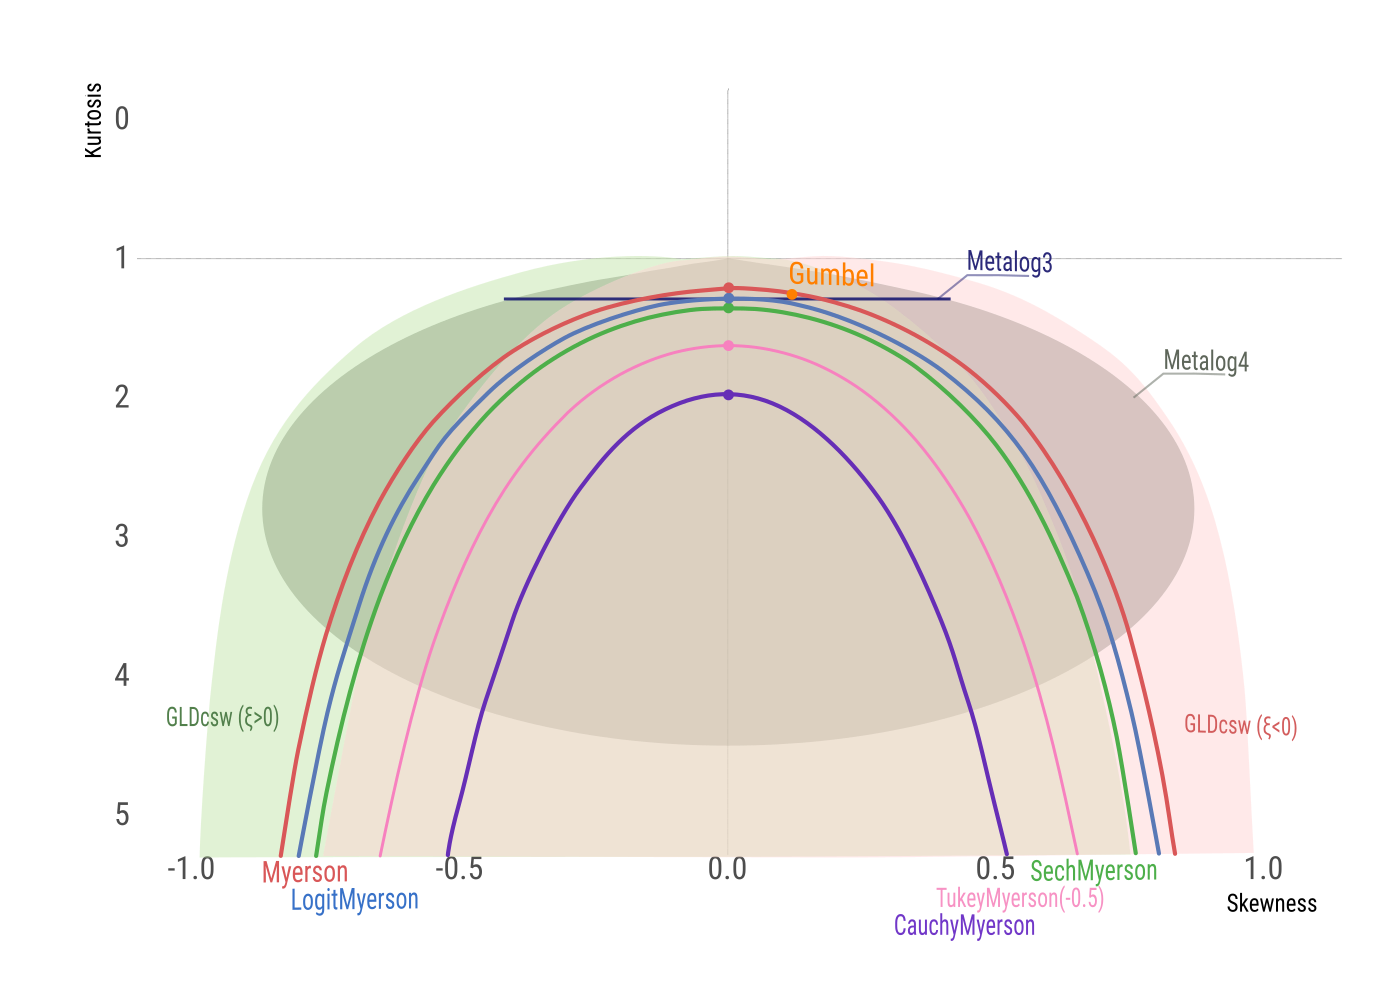
\includegraphics[width=0.8\textwidth,height=\textheight]{img/unbounded_final.png}

}

\caption{\label{fig-unbounded}Robust skewness vs robust kurtosis for
some unbounded distributions}

\end{figure}%

\begin{figure}

\centering{

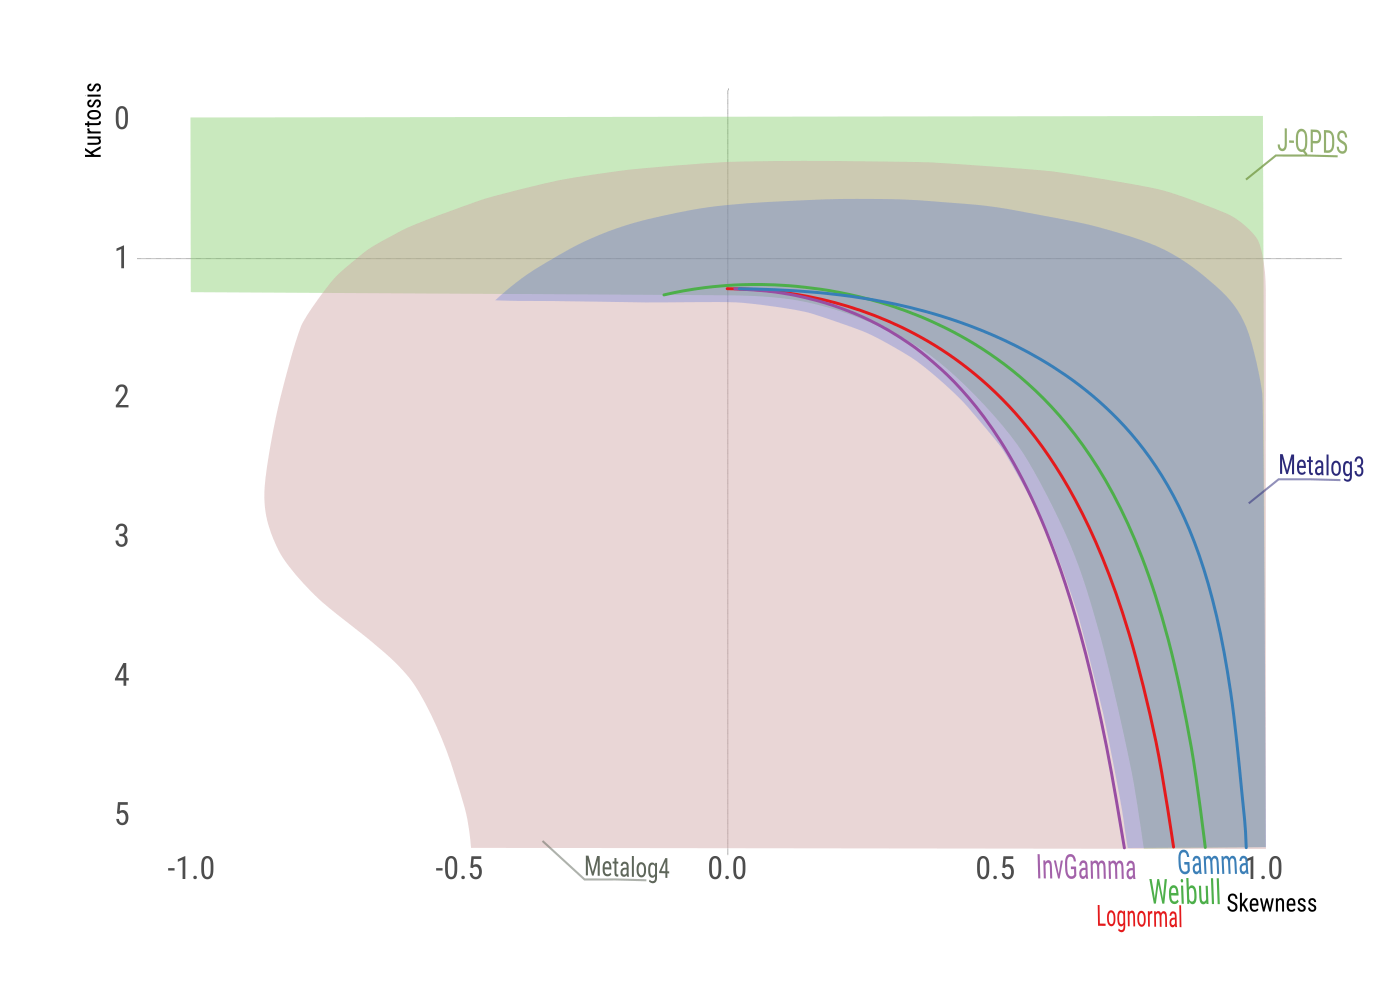
\includegraphics[width=0.8\textwidth,height=\textheight]{img/semibounded_final.png}

}

\caption{\label{fig-semibounded}Robust skewness vs robust kurtosis for
some left-bounded distributions}

\end{figure}%

\begin{figure}

\centering{

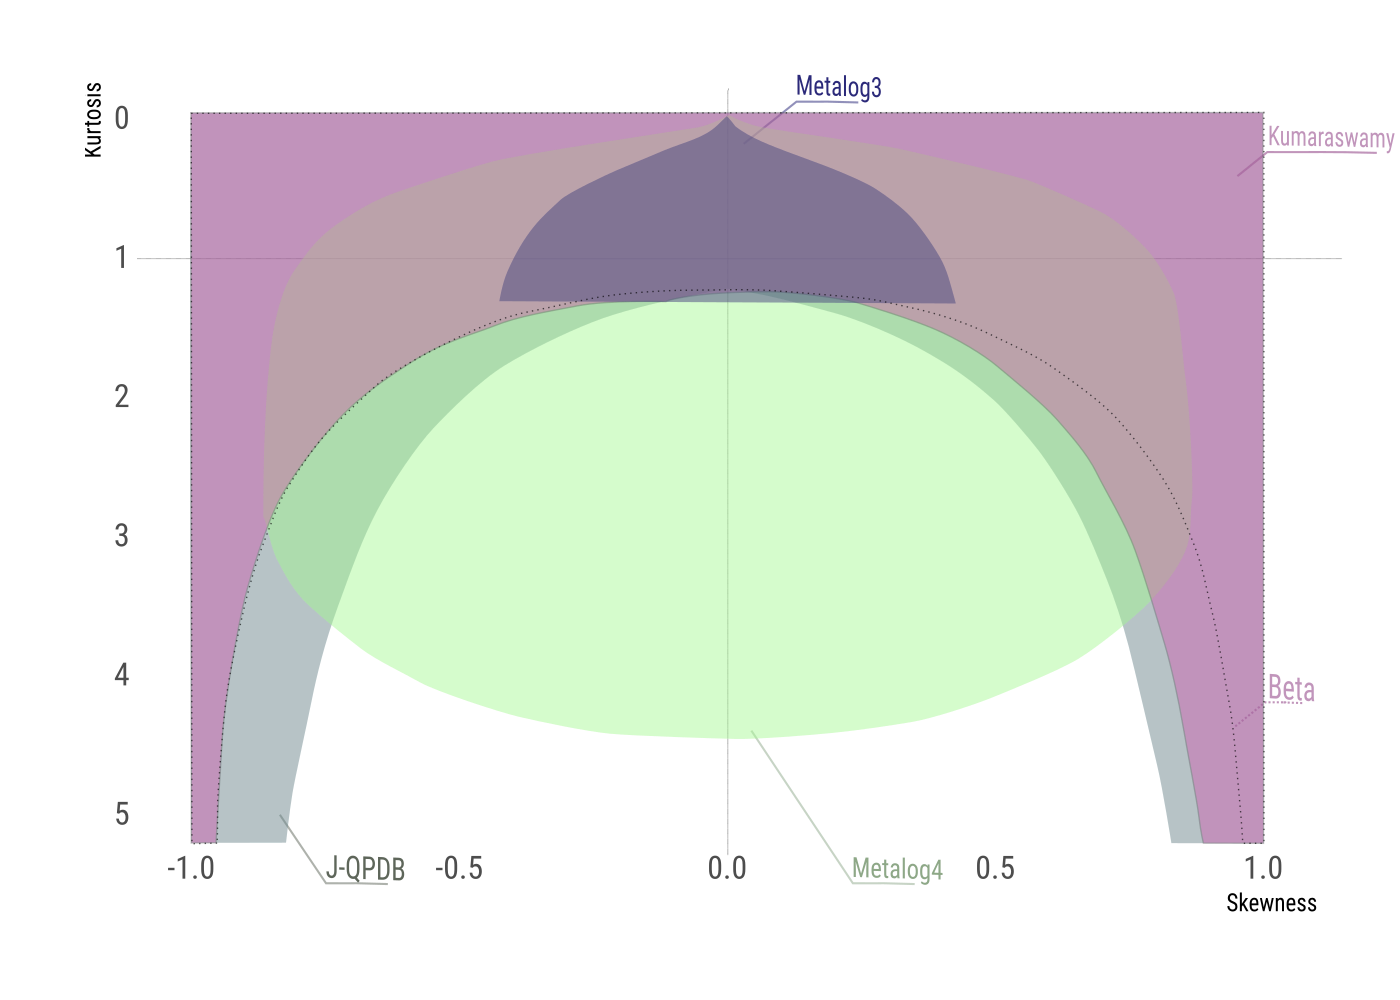
\includegraphics[width=0.8\textwidth,height=\textheight]{img/bounded_final.png}

}

\caption{\label{fig-bounded}Robust skewness vs robust kurtosis for some
bounded distributions}

\end{figure}%

\section{Multivariate quantile-parameterized
distributions}\label{sec-multivariateqpd}

Quantile-parameterized distributions can serve as marginal distributions
in multivariate models, where the dependency structure is captured by a
standard (parametric) multivariate distribution, a copula, or described
by bivariate quantiles. However, the marginal distributions alone are
insufficient to determine the corresponding bivariate distribution,
resulting in an infinite number of bivariate distributions with the same
margins
\citep{gumbel1960BivariateExponentialDistributions, gumbel1961BivariateLogisticDistributions}.
In this section, we describe several methods for extending the
distributions parameterized by the quantile-probability pairs to become
Multivariate Quantile-Parameterized Distributions (MQPDs).

\subsection{MQPDs based on standard multivariate
distributions}\label{mqpds-based-on-standard-multivariate-distributions}

\subsubsection{Normal distribution}\label{normal-distribution}

In the simplest case, multivariate Quantile-Parameterized Distributions
(MQPDs) can be created by using the multivariate normal distribution,
following the approach of \citep{hoff2007ExtendingRankLikelihood}. The
Myerson, J-QPD, and SQN quantile functions are Q-transformations of the
probit \(Q(z(u)\vert\theta)\), where \(z(u)=\Phi^{-1}(u)\) represents
the standard normal quantile function. The multivariate versions of
these distributions can be viewed as the Q-transformations of the
multivariate normal distribution. To extend these QPDs to \(J\)
dimensions using the multivariate normal distribution, we employ the
method outlined in \citep{drovandi2011LikelihoodfreeBayesianEstimation}.

The \(i\)-th component of a single observation \(y_i\) can be described
by the quantile function:

\[
y_i=Q(z(u_i)\vert\theta_i), \; \text{for }i=1,\dots,J 
\]

where \(\theta_i\) represents the set of parameters for component \(i\)
(e.g., \(\{q_1,q_2,q_3, \alpha\}_i)\) for Myerson or J-QPD
distributions). The vector \((z(u_1),\dots,z(u_j))^T\sim N(0,\Sigma)\),
where \(\Sigma\) denotes the covariance matrix.

For invertible distributions, the inverse quantile function is the
cumulative distribution function (CDF)
\(Q^{-1}(y_i\vert\theta)=F(y_i\vert\theta)\), otherwise, the inverse can
be computed numerically as
\(\widehat{F}(y_i\vert\theta)=\widehat{Q^{-1}}(y_i\vert\theta)\)
\citep{perepolkin2023TenetsQuantilebasedInference}.

Drovandi and Pettitt
\citep{drovandi2011LikelihoodfreeBayesianEstimation} show that the joint
density of a single (multivariate) observation \((y_i,\dots,y_J)\) can
be expressed as:

\[
\begin{gathered}
f(y_1,\dots,y_J\vert\theta)=\\
\varphi\left[z(Q^{-1}(y_1\vert\theta_1)),\dots,z(Q^{-1}(y_J\vert\theta_J));\Sigma\right]\times\\
\quad \times\prod_{i=1}^{J}\frac{dQ^{-1}(y_i\vert\theta_i)}{dy_i}
\end{gathered}
\]

where \(z(Q^{-1}(y_i\vert\theta_i))=z_i\),
\(\varphi(z_1,\dots,z_J;\Sigma)\) represents the multivariate normal
density with a mean of zero and a covariance matrix of \(\Sigma\), and
\(\frac{dQ^{-1}(y_i)}{dy_i}=f(y_i)\) is the probability density function
(PDF) of the QPD (refer to Appendix A).

For distributions without a PDF, the same joint density can be expressed
as a joint density quantile function

\[
\begin{gathered}
\\
[q(u_1,\dots,u_j)]^{-1}=\\
\varphi(z(u_1),\dots,z(u_J);\Sigma)\times\\
\quad \times \prod_{i=1}^{J}[q(u_i\vert\theta_i)]^{-1}
\end{gathered}
\]

since \(Q^{-1}(y_i\vert\theta_i)=u_i\) and
\(f(y_i\vert\theta_i)=[q(u_i\vert\theta_i)]^{-1}\)
\citep{gilchrist2000StatisticalModellingQuantile}.

It's worth noting that this method of creating multivariate
distributions does not require every component to follow the same
distributional form. As illustrated earlier, it is entirely possible to
combine several different QPDs using the multivariate Gaussian
distribution \citep{drovandi2011LikelihoodfreeBayesianEstimation}.

To use the MQPD for the prior, both the density of the multivariate
normal and the marginal densities need to be explicitly added to the
log-likelihood. This is possible when the marginal QPDs used to define
the multivariate prior are invertible, such as Myerson and J-QPD, as
both the CDF (\(Q^{-1}(y_i\vert\theta_i)\)) and PDF
(\(dQ^{-1}(y_i\vert\theta_i)/dy_i\)) are required.

When a quantile-based prior specification is used, only the multivariate
normal log-density needs to be added because the Jacobian for the
marginal QF transformation is reciprocal to the DQF of the prior
\citep{perepolkin2023TenetsQuantilebasedInference}.

\subsubsection{Logistic distribution}\label{logistic-distribution}

The same approach of joining the marginal QPDs can be applied by using
the base quantile functions of other distributions. For instance, the
Logit-Myerson distribution \citep{wilson2023ReconciliationExpertPriors}
is based on the logistic quantile function. Two Logit-Myerson
distributions can be connected using the bivariate logistic
distribution. \citep{gumbel1961BivariateLogisticDistributions} proposed
three different formulations for the bivariate logistic distribution.
The Type II distribution from the Morgenstern Family
\citep{sajeevkumar2014EstimationParameterMorgenstern, basikhasteh2021BayesianEstimationMorgenstern}
has the following joint distribution and density functions:

\[
\begin{aligned}
&F(y_1,y_2\vert\beta)=F_1(y_1)F_2(y_2)\times\\
&\quad \times [1+\beta(1-F_1(y_1))(1-F_2(y_2))]\\
&f(y_1,y_2\vert\beta)=f_1(y_1)f_2(y_2)\times\\
&\quad \times [1+\beta(1-2F_1(y_1))(1-2F_2(y_2))]
\end{aligned}
\]

where \(F_i(y_i)\) and \(f_i(y_i)\) for \(i\in\{1,2\}\) refer to the
univariate logistic distribution and density funcitons, respectively and
\(-1\leq\beta\leq1\). Since \(y_i=Q_i(u_i)\) we can express the
bivariate density in the quantile form

\[
\begin{gathered}
f(Q(u_1),Q(u_2)\vert\beta)=f_1(Q(u_1))f_2(Q(u_2))\times\\
\times [1+\beta(1-2F_1(Q_1(u_1)))(1-2F_2(Q_2(u_2)))]\\
\left[q(u_1,u_2\vert\beta)\right]^{-1}=[q_1(u_1)]^{-1}[q_2(u_2)]^{-1} \times\\
\times \left[1+\beta (1-2u_1)(1-2u_2)\right]
\end{gathered}
\]

For logistic distribution \(Q(u)=\ln(u)-\ln(1-u)\) and
\([q(u)]^{-1}=u(1-u)\). Therefore, the bivariate logistic density
quantile function can be expressed as

\[
\begin{gathered}
\left[q_L(u_1,u_2\vert\beta)\right]^{-1}=u_1(1-u_1)u_2(1-u_2)\times\\
\quad\times \left[1+\beta (1-2u_1)(1-2u_2)\right]
\end{gathered}
\]

If we combine the QPD marginals, the result is the joint quantile-based
density for the bivariate logistic-based QPD, where the dependency is
captured by the bivariate logistic distribution with the coupling
parameter \(\beta\), and the margins are QPDs. The joint density
quantile function is given by:

\[
\begin{gathered}
\left[q_{MQPD}(u_1,u_2\vert\theta_1,\theta_2, \beta)\right]^{-1}=\\
u_1(1-u_1)u_2(1-u_2)\times\\
\times\left[1+\beta (1-2u_1)(1-2u_2)\right]\times\\
\times [q_1(u_1\vert\theta_1)]^{-1}[q_2(u_2\vert\theta_2)]^{-1}
\end{gathered}
\]

Here, \([q_i(u_i\vert\theta_i)]^{-1}\), for \(i=1,2\), represents the
marginal QPD density quantile functions, such as the density quantile
function (DQF) of the Logit-Myerson distribution (see Appendix A).

\begin{figure}

\centering{

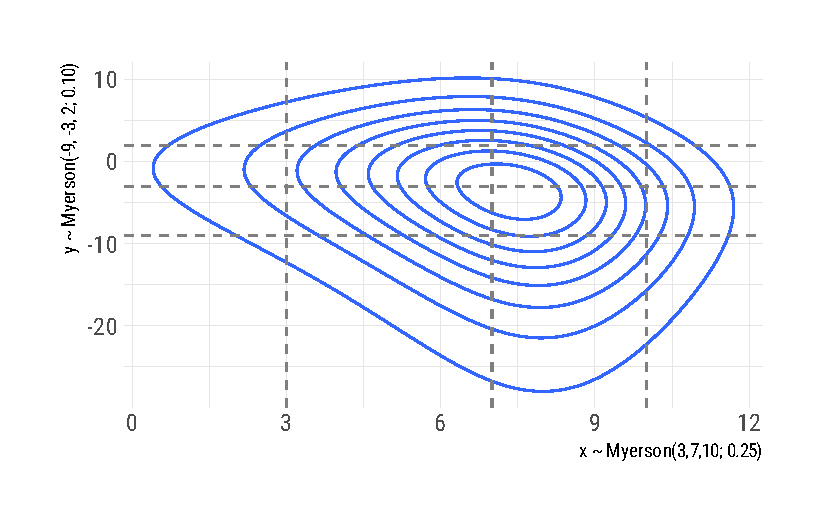
\includegraphics[width=0.8\textwidth,height=\textheight]{qpppp_files/figure-pdf/fig-bi-logitmyerson-1.pdf}

}

\caption{\label{fig-bi-logitmyerson}Density of Generalized Myerson
distributions joined by Type II bivariate logistic distribution}

\end{figure}%

Figure~\ref{fig-bi-logitmyerson} presents the Bivariate Logit-Myerson
Distribution, parameterized by \(\Theta=\{\theta_1, \theta_2, \rho\}\),
where the marginal Myerson distributions are given by
\(y_{ij}=Q_j(z(u_{ij}),\theta_j)\) for \(j=1,2\), with parameter vectors
\(\theta_1=\{3,7,10;0.25\}\), \(\theta_2=\{1,10,20;0.1\}\), and the
dependence parameter \(\beta=0.6\).

\subsection{Copula-based MQPDs}\label{copula-based-mqpds}

The approach we have used so far is similar to constructing the joint
distribution using the Gaussian copula
\citep{hoff2007ExtendingRankLikelihood}. Copulas provide a general
approach to modeling joint distributions, separating the bivariate
dependence from the effects of marginal distributions
\citep{kurowicka2006UncertaintyAnalysisHigh}. The literature describes a
wide range of copulas
\citep{genest2007EverythingYouAlways, smith2013BayesianApproachesCopula, kurowicka2011DependenceModelingVine},
and new copulas can be created using generator functions
\citep{durrleman2000SimpleTransformationCopulas}. When a copula is used
to connect QPDs, the joint density is calculated as follows:

\[
\begin{gathered}
f_{MQPD}(y_1,y_2\vert \theta_1,\theta_2,\Xi)=\\
c(F(y_1\vert\theta_1),F(y_2\vert\theta_2)\vert\Xi)\times \\
\times f_1\left(y_1\vert\theta_1\right) f_2\left(y_2\vert\theta_2\right)
\end{gathered}
\]

where \(c\) represents the copula density function with parameter
\(\Xi\), and \(F(y_i\vert\theta_i)\) and \(f_i(y_i\vert\theta_i)\) are
the CDF and PDF of the marginal quantile-parameterized distributions,
respectively.

The same density can be expressed in quantile-based form
\citep{perepolkin2023TenetsQuantilebasedInference}:

\[
\begin{gathered}\\
[q_{MQPD}(u_1,u_2\vert\theta, \Xi)]^{-1}=\\
c\left(u_1,u_2\vert\Xi\right)\times \\
\times [q_1(u_1\vert\theta_1)]^{-1}[q_2(u_2\vert\theta)]^{-1}
\end{gathered}
\]

where \(c\) is the copula density function with parameter \(\Xi\), and
\([q_i(u_i\vert\theta_i)]^{-1}\), for \(i=1,2\), are the marginal DQFs
of QPDs. Figure~\ref{fig-bc-myerson} presents 10,000 samples from the
bivariate Myerson distribution joined by the Joe copula with
\(\theta=3\).

Elicitation of multivariate distributions may require a specialized
approach
\citep{elfadaly2017ElicitingDirichletGaussian, wilson2021RecentAdvancesElicitation}.
For examples of expert-specified multivariate distributions encoded with
copulas, we refer to
\citep{wilson2018SpecificationInformativePrior, holzhauer2022ElicitingJudgementsDependent, sharma2018RegularizationVariableSelection, aas2009PaircopulaConstructionsMultiple}.
When fitting copulas to empirical observations, the ``blanket'' goodness
of fit measure \citep{wang2000ModelSelectionSemiparametric} based on
Kendall's transform
\citep{genest2006GoodnessofFitProceduresCopula, genest2009GoodnessoffitTestsCopulas}
can be used.

\begin{figure}

\centering{

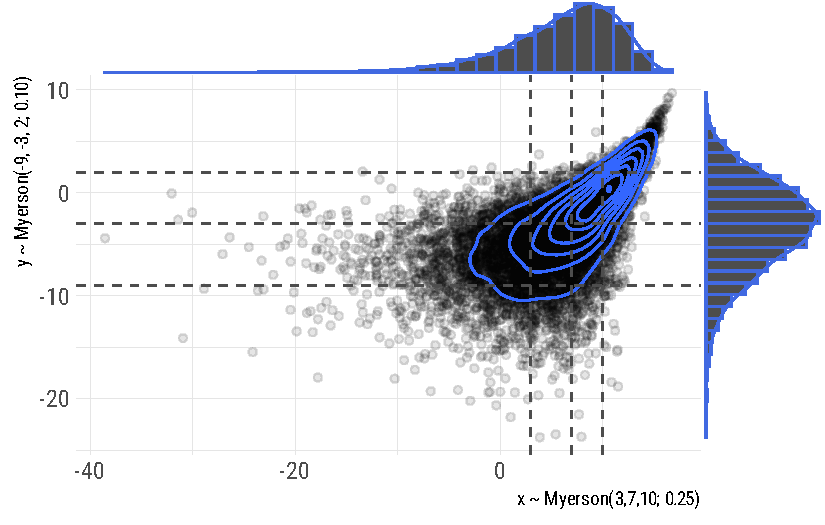
\includegraphics[width=0.8\textwidth,height=\textheight]{qpppp_files/figure-pdf/fig-bc-myerson-1.pdf}

}

\caption{\label{fig-bc-myerson}Samples from the bivariate Myerson
distribution joined by the Joe copula (\(\theta=3\))}

\end{figure}%

\subsection{Bivariate quantiles}\label{bivariate-quantiles}

The formal definition of bivariate quantile functions and the method for
constructing bivariate quantile distributions using marginal and
conditional quantile functions are provided by
\citep{nair2023PropertiesBivariateDistributions, vineshkumar2019BivariateQuantileFunctions}.
They define the bivarate quantile function (bQF) of \((X_1, X_2)\) as
the pair \(Q(u_1, u_2)=(Q_1(u_1), Q_{21}(u_2\vert u_1))\), where
\(Q_1(u_1)=\inf \{x_1: F_1(x_1)\geq u_1\}\), \(u_1\in[0,1]\) and
\(Q_{21}(u_2\vert u_1)=\inf\{x_2: F_{21}(Q_1, x_2)\geq u_2\}\).

The conditional quantile function \(Q_{21}(u_2\vert u_1)\) can be
obtained by inverting the conditional distribution function
\(F_{21}(x_1, x_2)\), which is computed from the factorization of the
joint survival function. The joint survival function is defined as
\(\bar{F}(x_1, x_2)=P(X_1> x_1)P(X_2> x_2 \vert X_1 > x_1)= \bar{F}(x_1)\bar{F}_{21}(x_1,x_2)\).
Note that the joint survival function
\(\bar{F}(x_1,x_2)=1-F_1(x_1)-F_2(x_2)+F(x_1,x_2)\), and the conditional
survival function \(\bar{F}_{21}(x_1,x_2)=1-F_{21}(x_1,x_2)\).

Another approach for creating bivariate quantile functions is through
Gilchrist's QF transformation rules
\citep{gilchrist2000StatisticalModellingQuantile}, which can be
generalized to bivariate quantile functions. According to
\citep{nair2023PropertiesBivariateDistributions} (Property 6), the
conditional QF can be constructed as a sum of two univariate QFs:
\(Q_{21}(u_2\vert u_1) = Q_1(u_1) + Q_2(u_2)\). This means that the pair
\((Q_1(u_1), ; Q_1(u_1) + Q_2(u_2))\) is a valid bivariate quantile
function, which generalizes Gilchrist's \emph{addition rule}
(Table~\ref{tbl-qf-trans}). The addition rule also works for quantile
density functions (Property 7). If \(Q_1\) is left-bounded at zero,
i.e., \(Q_1(0) = 0\), then the margins of such a bQF are
\(X_1 = Q_1(u_1)\) and \(X_2 = Q_2(u_2)\). Otherwise, the marginal
distribution of \(X_2\) will be
\(\lim_{u_1 \rightarrow 0}Q_{21}(u_2\vert u_1)\), which in many cases is
not tractable.

If \(Q_1(u_1)\) and \(Q_2(u_2)\) are positive on \(u_i \in [0,1]\), then
their product is also a valid conditional QF (Property 8), generalizing
Gilchrist's ``product rule''. Finally, Property 9 generalizes the
``Q-transformation rule,'' stating that for every increasing
transformation functions \(T_1\) and \(T_2\),
\(\left(T_1(Q_1(u_1)), T_1(Q_1(u_1)) + T_2(Q_2(u_2))\right)\) is also a
valid bQF.

Therefore, valid bivariate quantile-parameterized QFs can be created by
constructing the conditional quantile functions as Gilchrist
combinations of univariate quantile-parameterized QFs.
Figure~\ref{fig-bq-myerson} shows 1000 samples from the bivariate
distribution created by adding together two Myerson distributions. Note
that in this case, only the marginal distribution of \(x_1 = Q_1(u_1)\)
is available in closed form.

\[
\begin{aligned}
(u_1, u_2) &\overset{X_1, X_2}{\backsim} (Q_1(u_1), Q_1(u_1)+Q_2(u_2))\\
Q_1(u_1) &\sim\text{Myerson}(3,7,10; 0.1)\\
Q_2(u_2) &\sim \text{Myerson}(-9, -3, 2; 0.25)\\
\end{aligned}
\]

This bQF is easy to elicit and interpret, since \(Q_2(u_2)\) can be
thought of as a random adjustment to the value of \(Q_1(u_1)\). In fact,
the conditional quantile function \(Q_{21}(u_2\vert u_1)\) can be
thought of as having the classical form
\(Q_{21}(u_2\vert u_1) = \mu(u_1) + \sigma Q_2(u_2)\)
\citep{gilchrist2000StatisticalModellingQuantile}, where the location is
randomly varying with \(\mu(u_1) = Q_1(u_1)\) and the scale parameter
\(\sigma = 1\). First, the marginal distribution \(Q_1(u_1)\) is
elicited, and then the difference between the values \(x_1\) and \(x_2\)
can be elicited as a QPT and encoded as \(Q_2(u_2)\).

\begin{figure}

\centering{

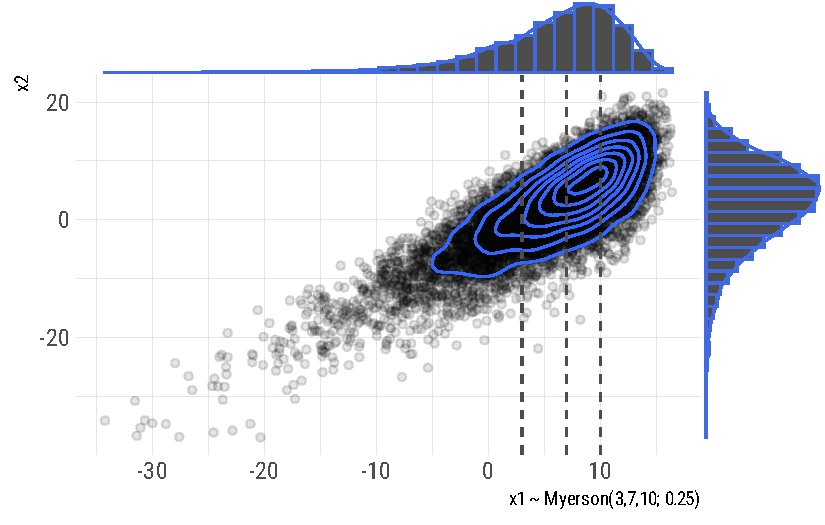
\includegraphics[width=0.8\textwidth,height=\textheight]{qpppp_files/figure-pdf/fig-bq-myerson-1.pdf}

}

\caption{\label{fig-bq-myerson}Samples from the Bivariate Myerson
quantile function}

\end{figure}%

\section{Discussion}\label{discussion}

Quantile-based distributions have garnered significant attention in the
research community. Several distributions, such as the Generalized
Lambda Distribution (GLD)
\citep{freimer1988StudyGeneralizedTukey, ramberg1974ApproximateMethodGenerating},
the g-and-k distribution
\citep{haynes1997RobustnessRankingSelection, haynes2005BayesianEstimationGandk, jacob2017LikelihoodCalculationGandk, prangle2017GkPackageGandk},
the g-and-h distribution
\citep{field2006MultivariateGandhDistribution, macgillivray1992ShapePropertiesGandh, rayner2002NumericalMaximumLikelihood},
and the Wakeby distribution
\citep{jeong-soo2005WakebyDistributionMaximum, rahman2015ApplicabilityWakebyDistribution, tarsitano2005FittingWakebyModel},
have been extensively studied and documented in the literature. These
distributions are defined by non-invertible quantile functions
\citep{perepolkin2023TenetsQuantilebasedInference}. However, the
research on quantile-parameterized distributions remains relatively
unexplored. These distributions offer interpretable parameters that are
defined on the same scale as the quantities of interest, simplifying the
elicitation process for experts. Many popular elicitation protocols for
both predictive and parametric elicitation rely on the assessment of
quantile-probability pairs (QPPs). Instead of fitting a parametric
distribution to the elicited QPPs
\citep{best2020PriorElicitation, ohagan2019ExpertKnowledgeElicitation},
assessors could directly use the elicited QPPs as inputs into one of the
QPD quantile functions, which can be easily employed in both
quantile-parameterized and parametric models.

Provided that the expert and the elicitor agree on the scientific model
to be used for representing the expert's understanding of the world
\citep{burgman2021ElicitingModelStructures}, several types of inputs may
be required to inform the model. Among those are the expert's judgement
about the model \emph{parameters}
\citep{mikkola2021PriorKnowledgeElicitation, ohagan2019ExpertKnowledgeElicitation}
and their \emph{predictions} of the next observation
\citep{akbarov2009ProbabilityElicitationPredictive, kadane1998ExperiencesElicitation, winkler1980PriorInformationPredictive}.
Both parametric and predictive judgments should be captured together
with corresponding uncertainties to reflect the expert's state of
knowledge. Quantile-parameterized distributions offer distinct
advantages as high-fidelity priors that precisely capture expert
assessments. These distributions are particularly beneficial for domain
experts who may not be well-versed in statistics, as they provide high
flexibility while retaining parameter interpretability. As a result,
QPDs can faithfully represent an expert's beliefs without compromising
convenience or precision.

Different quantile-parameterized distributions fitted to the same set of
quantile-probability pairs may exhibit slight variations in shape.
However, given the diverse range of QPDs proposed in the literature a
knowledgeable assessor should be able to select an appropriate
distribution and validate the choice with the expert, taking into
account the thickness of the distribution tails.

Most QPDs we reviewed are parameterized by a symmetric percentile
triplet (SPT). These distributions rely on the symmetric property of
underlying \emph{kernel} distributions and can be generalized by
swapping the distribution with another one that exhibits different tail
shapes. Hadlock and Bickel
\citep{hadlock2019GeneralizedJohnsonQuantileParameterized} utilized this
method to generalize Johnson Quantile Parameterized distributions
(J-QPDs). We show that the variants of Myerson distribution appearing in
the literature
\citep{myerson2005ProbabilityModelsEconomic, wilson2023ReconciliationExpertPriors}
represent similar generalization. This principle can be extended to
include other kernels which result in varying thickness of the tails.

\subsubsection*{Quantile function
perspective}\label{quantile-function-perspective}
\addcontentsline{toc}{subsubsection}{Quantile function perspective}

The distributions discussed in this paper are defined using the quantile
function and, therefore, they can be considered \emph{quantile-based}
quantile-parameterized distributions. Myerson, J-QPD, and several other
quantile-parameterized distributions reparameterize conventional
distributions, utilizing Gilchrist's Quantile Function (QF)
transformations \citep{gilchrist2000StatisticalModellingQuantile}.

Perepolkin et al. \citep{perepolkin2023TenetsQuantilebasedInference}
demonstrated that the distributions defined by the quantile function can
be used both as prior and as likelihood in Bayesian models. Priors
defined by the quantile function eliminate the need to compute prior
density. The quantile function acts as a non-linear transformation of a
uniform degenerate random variate with the resulting Jacobian adjustment
reciprocal to the density quantile function. Therefore, both the
Jacobian and the density quantile function are omitted from the Bayesian
updating equation \citep{perepolkin2023TenetsQuantilebasedInference}.
When using quantile-based QPDs as likelihood, special care needs to be
taken with regards to the suitable prior for the QPP parameters.
\citep{perepolkin2021HybridElicitationIndirect} used the Dirichet-based
prior for the metalog likelihood model and descibed the \emph{hybrid}
elicitation process for encoding the expert judgments into the
two-dimensional prior distribution implied by the model.

\subsubsection*{Feasibility of
parameters}\label{feasibility-of-parameters}
\addcontentsline{toc}{subsubsection}{Feasibility of parameters}

Not all QPDs are equally reliable in approximating the underlying
distributions. Violating the QF transformation rules imposes additional
constraints on the feasibility of parameters, as certain combinations of
parameters may result in locally decreasing quantile functions
\citep{keelin2016MetalogDistributions, hadlock2017QuantileparameterizedMethodsQuantifying}.
We discussed this limitation in relation to SQN and metalog
distributions, but the same challenges affect other distributions with
QF violating Gilchrist QF transformation rules. In this regard, the
quantile-parameterized model, which relies on Gilchrist combination of
basic quantile functions, proposed by
\citep{peng2023MixtureQuantilesEstimated}, represents a highly promising
advancement. Weighted constrained optimization algorithm ensuring that
the quantile mixture weights remain non-negative opens new possibilities
for other QPDs using monotonic transformations of quantile functions.
The estimator proposed by \citep{peng2023MixtureQuantilesEstimated} is
asymptotically a q-Wasserstein distance, which has also been used for
parameter estimation in Approximate Bayesian Computation
\citep{bernton2019ParameterEstimationWasserstein}.

The feasibility conditions for the Generalized Lambda Distribution (GLD)
have been a focal point of numerous research endeavors in the past
\citep[etc]{dean2013ImprovedEstimationRegression, fournier2007EstimatingParametersGeneralized, karian2019FittingStatisticalDistributions, king2007FittingGeneralizedLambda, tarsitano2005EstimationGeneralizedLambda}.
Various reparameterizations have been explored to enhance parameter
identifiability \citep{ramberg1974ApproximateMethodGenerating}.
Recently, \citep{chalabi2012FlexibleDistributionModeling} proposed a
novel asymmetry-skewness reparameterization for the previously popular
Freimer, Kollia, Mudholkar \& Lin version of GLD (FKML GLD)
\citep{freimer1988StudyGeneralizedTukey}, wherein two of the four
parameters are mapped to robust quantile-based moments, namely the
median and Interquartile Range (IQR). This reduction in the number of
parameters required for data fitting simplifies the previously
computationally intensive fitting algorithms. As demonstrated in the
plot of robust moments (Figure~\ref{fig-unbounded}) GLD remains one of
the most flexible unbounded distributions, capable of accommodating a
wide range of shapes.
\citep{dedduwakumara2021EfficientEstimatorParameters} described a
two-step method for fitting FKML GLD using the probability density
quantile function \citep{staudte2017ShapesThingsCome}. However, when
applying their method to fitting the CSW GLD, the second step becomes
unnecessary as the location and scale can be directly mapped to the
empirical first and second robust moments.

CSW GLD represents a prime example of clever reparameterization aiming
at alleviating the deficiencies of QF construction through setting
consistent parameter boundaries and defining fall-back cases for an
impossible combination of parameters. This degree of reparameterization
is difficult for QPDs because the objective is to retain the mapping of
parameters to the valid set of quantile-probability pairs. Therefore,
for improperly constructed QPDs the feasibility conditions will have to
be expressed as ratios of quantiles.

\subsubsection*{Multivariate extensions}\label{multivariate-extensions}
\addcontentsline{toc}{subsubsection}{Multivariate extensions}

Quantile-parameterized distributions can be readily extended to the
multivariate setting by leveraging traditional multivariate
distributions. The combination of quantile-based marginal distributions
joined by the multivariate normal has been previously discussed in the
literature
\citep{drovandi2011LikelihoodfreeBayesianEstimation, hoff2007ExtendingRankLikelihood}.
Building on this approach, we proposed the use of Gumbel's bivariate
logistic distribution \citep{gumbel1961BivariateLogisticDistributions}
to combine quantile-parameterized Logit-Myerson distributions
\citep{wilson2023ReconciliationExpertPriors}.

Copulas offer a natural extension of univariate QPDs into the
multivariate domain. Bivariate copulas can be assembled into more
complex structures using vine copulas
\citep{czado2019AnalyzingDependentData, kurowicka2011DependenceModelingVine, wilson2018SpecificationInformativePrior}.
Flexible QPDs serve as a viable alternative to empirical copulas, where
the margins are represented by kernel density estimation (KDE) or other
non-parametric approaches. Poorly fitted marginal distributions mean
\emph{less-than-ideal} starting point for copula modeling, because of
deviations from uniformality of the copula margins.

Quantile-parameterized distributions defined by the quantile function
are particularly well-suited for constructing new distributions using
bivariate quantiles
\citep{nair2023PropertiesBivariateDistributions, vineshkumar2019BivariateQuantileFunctions}.
The ability to construct a conditional quantile function as a Gilchrist
combination of univariate quantile functions offers a convenient and
interpretable approach to defining bivariate distributions, especially
when the univariate quantile functions are parameterized by quantiles.
These distributions are easy to sample from and construct. However,
fitting these distributions to data or posterior samples can be
challenging. As shown by \citep{castillo1997FittingContinuousBivariate}
the fitting process requires all marginal and conditional quantile
functions to be available in closed form, which is often unattainable.

\subsubsection*{Further research}\label{further-research}
\addcontentsline{toc}{subsubsection}{Further research}

There appears to be a limited availability of unbounded
quantile-parameterized distributions in the current literature. Among
the distributions we examined, only the metalog distribution and
quantile mixtures can extend across the entire real line. The G-QPD
system provides clear distributional bounds explicitly defined by the
expert during elicitation. In contrast, the (Generalized) Myerson
distribution system relies on implicit bounds that need to be
communicated to the expert. Most of the distributions we reviewed are
characterized by a symmetrical percentile triplet (SPT), as they rely on
the symmetrical property of their kernels. However, there may be
situations where an arbitrary (non-symmetrical) quantile
parameterization could prove valuable \citep[as shown
by][]{perepolkin2021HybridElicitationIndirect}. The development of
flexible quantile-parameterized distributions defined by an arbitrary
set of quantile-probability pairs using quantile mixtures
\citep{peng2023MixtureQuantilesEstimated} can enhance versatility of
QPDs and facilitate their broader adoption.

In conclusion, quantile-parameterized distributions offer a valuable
framework for capturing expert assessments and incorporating them into
statistical models. They provide high flexibility and parameter
interpretability, making them particularly beneficial for domain
experts. The diverse range of quantile-parameterized distributions
explored in the literature allows for customized modeling approaches
that align with the expert's beliefs and uncertainties. By embracing
these innovative distributions, researchers and practitioners can
enhance the accuracy and reliability of their statistical models while
leveraging expert knowledge effectively.

\section*{Miscellaneous}\label{miscellaneous}
\addcontentsline{toc}{section}{Miscellaneous}

\subsection*{Acknowledgments}\label{acknowledgments}
\addcontentsline{toc}{subsection}{Acknowledgments}

The authors have no conflict of interest to declare. We thank the
editorial team and reviewers for their constructive feedback which
helped us improve this manuscript.

\subsection*{ORCID}\label{orcid}
\addcontentsline{toc}{subsection}{ORCID}

Dmytro Perepolkin https://orcid.org/0000-0001-8558-6183\\
Erik Lindström https://orcid.org/0000-0002-6468-2624\\
Ullrika Sahlin http://orcid.org/0000-0002-2932-6253

\section*{References}\label{references}
\addcontentsline{toc}{section}{References}

\renewcommand{\bibsection}{}
\bibliography{qpppp-article.bib}




\end{document}
